\chapter[EXPLANATION OF TERMS, \&C. USED IN SHIP-BUILDING]{CHAPTER 1. \\
\footnotesize \singlespacing AN EXPLANATION OF THE TERMS, AND SOME ELEMENTARY PRINCIPLES, REQUISITE TO BE UNDERSTOOD IN THE THEORY AND PRACTICE OF SHIP-BUILDING.}

\textbf{ABAFT}. The hinder part of a ship, or toward the stern. 

\textbf{ABOARD}. Within, or upon, a ship. 

\textbf{ABREAST}. Alongside of, or opposite to; as in the case of two or more ships lying with their sides parallel, and their heads equally advanced. With regard to objects within the ship, this term implies on a line parallel with the beam, or at right angles with the ship's length; as "the \textsc{Fenders} should be placed abreast, or by the side of, the main hatchway."

\textbf{ABSCISSE}. See Conic SECTIONS. 

\textbf{ACUTE ANGLE}. See \textsc{Angle}. This sort of angle upon wood, \&c. is by shipwrights denominated an under bevelling. See \textsc{Bevelling}. \textit{See also Circle, Fig. 2. Plate A.}

\textbf{AFLOAT}. Borne up by, or floating in, the water.

\textbf{AFORE}. The fore part of a ship, or toward the stem. 

\textbf{AFT}. Towards, or near, the stern. 

\textbf{AFTER-BODY}. That part of a ship's body abaft the midships or dead-flat. (\textit{See} \textsc{Bodies}.) This term is more particularly used in expressing the \textit{figure} or \textit{shape} of that part of the ship. \textit{See Body Plan, Plate 1.} 

\textbf{AFTER PART OF THE SHIP}. All that part towards the stern, from the \textsc{Dead-flat}, or B broadest part of the ship. Or, with regard to the respective position of things placed in the direction of the ship's length, the term After denotes that which is nearest to the stern. 

\textsc{AFTER TIMBERS}. All those timbers abaft the \textsc{midships of dead flat}. 

\textsc{AHEAD}. Any thing, which is situated on that point of the compass to which a ship’s stem is directed, is said to be ahead of her. Objects on board are said to be taken \textit{ahead} when removed towards the stem. 

\textbf{AIR FUNNEL}. A cavity framed between the sides of some timbers, to admit fresh air into the ship, and convey the foul air out of it. \textit{See Disposition, Plate 3}. 

\textbf{AMIDSHIPS}. In midships, or in the middle of the ship, either with regard to her length or breadth. Hence that timber or frame which has the greatest breadth and capacity in the ship is denominated the \textit{midship bend}. See \textsc{Dead-Flat}. \textit{See also Sheer Draught, Plate 1.} 

\textbf{ANCHOR}. The instrument of iron, \&c. used, by means of a cable, to retain the ship in her station. 

\textbf{ANCHOR-LINING}. The short pieces of plank, or of board, fastened to the sides of the ship, or to stantions under the fore channel, to prevent the bill of the anchor from wounding the ship's side, when fishing the anchor. \textit{See Sheer Draught, Plate 1}. 

\textbf{To ANCHOR STOCK}. To work planks in a manner resembling the stocks of anchors, by fashioning them in a tapering form from the middle, and working or fixing them over each other, so that the broad or middle part of one plank shall be immediately above or below the butts or ends of two others. This method, as it occasions a great consumption of wood, is only used where particular strength is required, as in the \textsc{Spirkettings} under ports, \&c. 

\textbf{AN-END}. The position of any mast, \&c. when erected perpendicularly on the deck. The topmasts are said to be \textsc{an-end} when they are hoisted up to their usual stations. This is also a common phrase for expressing the driving of any thing in the direction of its length, as to force one plank, \&c. to meet the butt of another. 

\textbf{ANGLE}. A corner or point where two lines or two planes meet; as the lines AB and CB.
\begin{wrapfigure}{r}{0.4\textwidth}
\begin{center}
\begin{tikzpicture}
\draw(-2,0) -- (2,0) node[pos=-0.1]{C} node[pos=1.1]{D};
\draw(0,0) -- (0,2) node[pos=-0.2]{B} node[pos=1.1]{A};
\draw(0,0) -- (2,-1) node[pos=1.1]{E};
\draw[dashed](-1.5,0) arc[radius=1.5,start angle= 180, end angle=90];
\end{tikzpicture}
\end{center}
\end{wrapfigure}
An Angle is sometimes denoted by the single letter placed at the angular point, as B, or by three letters, of which that in the middle denotes the angle, as ABC. They are measured by the arch of a circle described from the centre with any radius, and are said to be greater or less according to the length of the arc contained between the legs or sides. If an angle contains exactly 90 degrees, (the one-fourth of the number of degrees in which every circle is supposed to be divided,) it is formed by one line perpendicular to another, and is called a \textsc{Right Angle}, as ABC or ABD. If containing more than 90 degrees, it is said to be an \textsc{Obtuse-Angle}, as CBE. If less than 90 degrees, an \textsc{Acute-Angle}, as DBE. An \textsc{Oblique-Angle} is a common name for any angle that is not a right one, whether acute or obtuse. \textit{See Circle, Plate A. }

\textsc{Angle} of \textsc{Direction}. That angle which is comprehended between the lines of direction of two conspiring forces; as of wind and tide. 

\textsc{Angle} of \textsc{Elevation}. That angle which is comprehended between a line of direction and any plane on which the projection is supposed to be made; as the angle formed by the direction of the bowsprit with the plane of the horizon. 

\textsc{Angle} of \textsc{Incidence}. The angle made with the line of direction, by an impinging body, at the point of impact; as that formed by the direction of the wind upon the sails, or of the water upon the rudder, of a ship. \textit{See} \textsc{Impulsion}. See also \textit{Fig. 2. Plate A}. 

\textsc{Angle} of \textsc{Obliquity}. See \textsc{Impulsion}. 

\textbf{APRON}. A kind of false or inner stem, fayed on the aftside of the stem, from the head down to the dead-wood, in order to strengthen it. It is immediately above the foremost end of the keel, and conforms exactly to the shape of the stem, so that the convexity of one applied to the concavity of the other forms one solid piece, which adds strength to the stem, and more firmly connects it with the keel. \textit{See Inboard Works, Plate 4}. 

\textbf{ARCH}. Any part of the circumference of a circle. But, although in Geometry an arc is generally so considered, yet, in Mechanics , or building, this term is applied to any regular curve, whether circular or elliptical, either for support or for ornament. Thus the beams of a ship, that support the decks and expand the sides, are said to be arched , or curved upwards, in their greatest length, equal to the round - up given in the Tables of Dimensions. And, as the beams are arches of circles, which cannot, from the great length of their radii, be struck from a centre, here follows the most correct way of obtaining that arch or round-up to which the beam mold must be made. See \textit{Fig. 1. Plate A}. 

First, strike the right line AB, equal to the length of the longest beam ; then erect or square up the line C in the middle of the line AB, and on it set-off the round - up of the beam as given in the dimensions. Then strike the lines AD, BD. With the radius CD, from the centre D, describe a circle, and make the arch a e equal to the arch Ca; and the arch bf equal to the arch Cb. So the arches a e, and bf, will be equal, and, of consequence, the angles ADC, ADe, BDC and BDf, will all be equal. 

Secondly, Divide the lines DC, De, and Df, into so many parts as shall be equal in number to the points of intersection required for the delineation of the required curve or arch. These parts may be either equal or unequal. It is only necessary that the divisions on the three lines, from the centre D, correspond with each other. 

Thirdly, Strike the line Bk to the first division of the line Df, and a line from A through b, (the first division of the line DC,) to intersect the line B in P, which will be one point in the required curve. In like manner the other points are found, by striking lines from B to the several divisions of the line Df, and lines from A through the corresponding divisions of the line DC, to intersect those drawn from B, which will be in the circumference of the circle or arch. In the figure, as it is small, we have only drawn the lines Bk and AP, in order to prevent confusion in its appearance: but, in practice, we may take two chalked lines, and fasten one at A and the other at B, and stretching the one through the spots in the line DC, and the other through the corresponding spots in Df or De, the intersections of the chalked lines will give the several points or spots in the circumference, and a batten then pinned to those spots will form the ticked curve ADB, to which the round-up is to be made. In the same manner may the round-up and round-aft moulds of the \textsc{Counter-Rails}, \&c. be made with more advantage than by any other method; because intersections may be obtained under the line AB, and the arch continued even to a circle, if required \footnote{For the satisfaction of the geometrical reader, a DEMONSTRATION of this problem is here subjoined. As the angle formed at the centre of a circle is measured by the opposite arch, so the angle formed at the circumference is measured by half the opposite arch. Hence all angles that stand on a similar chord are equal; and, consequently, if there be ever 80 many equal angles standing on a similar chord, they will be all in the circumference of a circle; or, what is the same thing, a curve drawn through the several angular points will be an arch of a circle. The triangles BDk and ADI are equal ; for the sides AD and DB are equal, the sides Dk and Dl are likewise equal, and the angle BDk included by the sides BD and Dk is equal to the angle ADI included by the sides AD and Di. Therefore the angle DBk is equal to the angle DAI. The angles DAB and DBA are equal; and, as the three angles of every triangle contain 180 degrees, subtracting their sum from 180, we have the angle ADB. But the sum of the angles kBA and IBA is equal to the sum of the angles DAB and DBA, for the angle DBk is added to the angle DBA, and the angle DAI (equal to the angle DBk) is subtracted from the angle DAB, therefore the angle AbB is equal to the angle ADH, and, of consequence, the arch of the circle will pass through both : the like of all the rest.}. 

\textsc{Equal Arches} are those which contain the same number of degrees, and whose radii are equal. 

\textsc{Similar Arches} are those which contain the same number of degrees, but whose radii may be unequal. For example. If the arch BC (\textit{Fig. 2. Plate A.}) contains the same number of degrees as the arch DE, or if the radius A B is to the radius AD as the arch BC is to the arch DE, then these arches are similar . 

\textbf{ARCH OF THE COVE}. An elliptical moulding sprung over the cove at the lower part of the taffarel. \textit{See Perpendicular View of the Stern in Plate 1}. 

\textbf{AREA}. The superficial content of any figure, as of a parallelogram, six feet long and four feet broad, whose area will be 24 feet, because 6 x 4 = 24. 

\textbf{ASTERN}. Any distance behind the ship, as opposed to \textsc{Ahead}. Objects on board are said to be \textit{astern} when near the stern of the ship. 

\textbf{ATHWART}. At right angles with the ship's length, or across the line of her course. 

\textbf{AVAST!} The command to stop or cease in any operation, as in bowsing or hawling. 

\textbf{AXIS}. A real or supposed line through the centre of a body, about which it may turn: and hence the revolving figure may be imagined to produce a solid. Thus, if a semi-circle be supposed to move round its diameter at rest, it will generate a sphere, the \textit{axis} of which is that diameter, and is commonly called the \textit{Axis of Rotation}. 

\textsc{Axis} is yet more generally used for a right line conceived to be drawn from the vertex of a figure to the middle of the base ; as the axis of a cone. See \textsc{Conic Sextions}. 

In Mechanics, the \textsc{Axis} of a \textsc{balance} is that line about which it moves or turns. The \textsc{Axis} of \textsc{Oscillation} is a right line, parallel to the horizon, passing through the centre, about which a pendulum vibrates. 

\textbf{AXIS} in \textbf{PERITROCHIO}, or \textsc{Wheel} and \textsc{Axle}. One of the five mechanical powers, on the principle of which are constructed the windlasses and capstans of ships. \textit{See} \textsc{Mechanics}, 

\textbf{BACK of the Post}. The after-face of the \textsc{Stern Post}. 

\textbf{BACK-STAYS}. The long ropes used to support the topmasts, \&c. and second the efforts of the shrouds when the mast is strained by a press of sail in a fresh wind. They reach from the topmast-heads to the starboard and larboard sides of the ship, where they are extended to the channels, or Backstay Stools. \textit{See Steel's "Art of Rigging."}   

\textbf{BACKSTAY STOOL}. A short piece of broad plank, bolted edge-ways to the ship's side, in the range of the channels, to project, and for the security of, the dead-eyes and chains for the Backstays. Sometimes the channels are left long enough to answer the purpose . See \textit{Sheer Draught, Plate 1.} 

\textbf{BACK-SWEEP}. See \textsc{Frames}. 

\textbf{BADGE}. A sort of ornament fixed on the quarters of small vessels near the stern, containing either a sash for the convenience of the cabin, or the representation of it. It is commonly decorated with carved work, such as marine figures, martial instruments, \&c. \textit{See Yacht , Plate 11}. 

\textbf{BALCONY}. The gallery in the stern of large ships. \textit{See Sheer Draught , and Perpendicular View of the Stern, Plate 1}. 

\textbf{BALANCE FRAMES}. Those frames , or bends of timber, of the same capacity or area, which are equally distant from the centre of gravity. See \textsc{Frames}. 

\textbf{BALLAST}. A quantity of iron, stone, or gravel, or such like materials, deposited in a ship's hold, when she has no cargo, or too little to bring her sufficiently low in the water. It is used to counterbalance the effort of the wind upon the sails, and give the ship a proper stability, that she may be enabled to carry sail, without danger of over-setting. 

\textbf{BALUSTERS}. The ornamental pillars placed in front of the balcony in the stern and quarters in large ships. 

\textbf{BARK}. A name given to small ships; especially to square-sterned ships having no headrails, and to such as have three masts without a mizen top sail. 

\textbf{BARREL}. The main piece of a capstan or steering wheel. See \textsc{Capstan} and \textsc{Steeringwheel}. \textit{See also Capstan, Plate 7}. 

\textbf{BARGE}. \textit{See} \textsc{Boats}. 

\textbf{BARS of the} \textsc{Capstans} \textbf{and} \textsc{Ports}. \textit{See} those Articles. 

\textbf{BASE}. The foot or lowest part of a pillar ; or that part of a body on which it rests, or is designed to rest. In geometry, an horizontal line upon which any figure is to be raised. 

\textit{The base of any surface as exposed to a stream of fluid} is that portion of a plane,
\begin{wrapfigure}{r}{0.4\textwidth}
\begin{center}
\begin{tikzpicture}
\draw[dotted](0,2) -- (4.4,2) node[pos=0, align=center, above]{D};
\draw[dotted](0,0) -- (4.4,0);
\draw(2,0) -- (4,2) node[pos=0, align=center, below]{B} node[pos=1, align=center, above]{A};
\draw(4,0) -- (4,2);
\draw(2,0) -- (4,0) node[pos=1, align=center, below]{C};
\draw[ultra thick, ->](0,1) -- (2,1);
\end{tikzpicture}
\end{center}
\end{wrapfigure} 
perpendicular to the stream, which is covered or protected from the action of the stream by the surface exposed to its impulse. Thus the base of a sphere exposed to a stream of fluid D. is its great circle, whose plane is perpendicular to the stream. Hence, if the plane surface AB was exposed to the action of a stream moving in the direction DA, then AC, perpendicular to BC, is its base. 

\textbf{BATTENS}. In general, light scantlings of wood. In ship-building, long narrow laths of fir, their ends corresponding and fitted into each other with mortice and tenon, used in setting fair the sheer-lines on a ship. They are painted black in order to be the more conspicuous. Battens used on the mold-loft floor, are narrow laths, of which some are accurately graduated and marked with feet, inches, and quarters, for setting off distances. Battens for gratings are narrow thin laths of Oak. See \textsc{Gratings}. 

\textbf{BEAK-HEAD}. The short platform at the fore part of the upper deck, in large ships, placed at the height of the ports from the deck, for the convenience of the chace-guns. Its termination aft is the bulk-head called the \textit{beak-head bulk-head}, which incloses the fore-part of the ship. \textit{See Sheer Draught, Plate 1}. 

\textbf{BEAK-HEAD-BEAM}. The same as \textsc{Cat-Beams}, which see.

\textbf{BEAMS}. The substantial pieces of timber which stretch across the ship, from side to side, to support the decks and keep the ship together by means of the \textit{Knees}, \&c. their ends being lodged on the clamps, keeping the ship to her breadth. \textit{See Plans of the Decks, Plates 5 and 6}. 

\textsc{Beam-Arm}, or \textsc{Fork-Beam}, is a curved piece of timber, nearly of the depth of the beam, scarphed, tabled, and bolted, for additional security to the sides of beams athwart large openings in the decks, as the main hatchway and the mast-rooms. \textit{See Plans of the Decks, Plates 5 and 6}. 

\textsc{Breast-Beams}. Are those beams at the fore-part of the quarter deck and roundhouse, and after part of the forecastle. They are sided larger than the rest; as they have an ornamental rail in the front, formed from the solid, and a rabbet one inch broader than its depth, which must be sufficient to bury the deals of the deck, and one inch above for a spurn-water. To prevent splitting the beam in the rabbet, the nails of the deck should be crossed, or so placed, alternately, as to form a sort of zigzag line. \textit{See Inboard Works, Plate 4, and Plans, Plate 6}. 

\textsc{Cat Beam}, or \textsc{Beak-Head Beam}. This is the broadest beam in the ship, generally made in two breadths, tabled and bolted together. The foreside is placed far enough forward to receive the heads of the stantions of the beak-head bulk-head. \textit{See Inboard Works, Plate 4, and Plans, Plate 6}. 

The \textsc{Collar-Beam} is the beam upon which the stantions of the beak-head hulk-head stand. The upper side of it is kept well with the upper side of the upper deck port-sills, and lets down upon the spirketting at the side. But its casting over the bowsprit in the middle giving it a form which in timber is not to be gotten without difficulty, a framing of two large carlings and a stantion on each side of the bowsprit is now generally substituted in its place. \textit{See Inboard Works, Plate 4}. 

\textsc{Half-Beams} are short beams introduced to support the deck where there is no framing, as in those places where the beams are kept asunder by hatchways, ladder ways, \&c. They are let down on the clamp at the side, and near midships into fore and aft carlings. On some decks they are, abast the mizen-mast, generally of fir, let into the side tier of carlings. S\textit{ee Plan of Upper Deck , Plate 6}. 

The \textsc{Midship Beam} is the longest beam of the ship, lodged in the midship-frame, or between the widest frame of timbers. 

\textsc{Palletting-Beams}, are those beams under the flat of the Magazine, Bread Room, and Powder Room, where there is a double \textit{palleting}. The upper tier are of fir, and rabbets are taken out of their edge to form scuttles. \textit{See Inboard Works, Plate 4, and Orlop Plan, Plate 5.} 

\textbf{BEARDING}. The diminishing of the edge or surface of a piece of timber, \&c. from a given line, as on the deadwood, clumps, plank-sheers, fife-rails, \&c. \textit{See Sheer Draught, Plate 1}

\textbf{BEARDING-LINE}. A curved line occasioned by bearding the dead wood to the form of the body; the former being sided sufficiently, this line is carried high enough to prevent the heels of timbers from running to a sharp edge, and forms a rabbet for the timbers to step on; hence it is often called the \textsc{Stepping Line}. \textit{See Sheer Draught, Plate 1.} 

\textbf{BED}. A solid framing of timber to receive and to support the mortar in a Bomb Vessel. 

\textbf{BED} or \textbf{BARREL SCREWS}. See \textsc{Screws}. 

\textbf{BEETLE}. A large mallet used by Caulkers for driving in their reeming irons to open the seams, in order for caulking.

\textbf{BELLFRY}. An ornamental framing, made of stantions, at the after beams of the forecastle, with a covering or top, under which the ship’s bell is hung. In large ships the stantions are supported by knees. In small ships it is sometimes built over the windlass. \textit{See Inboard Works, Plate 4}. 

\textbf{BELLY}. The inside or hollow part of compass or curved timber, the outside of which is called the BACK. 

\textbf{BELL-TOP}. A term applied to the top of a quarter gallery when the upper stool is hollowed away, or made like a rim, to give more height as in the quarter galleries of small vessels, and the stool of the upper finishing comes home to the side, to complete overhead. See the \textit{Draught of the Sloop, Plate 10}. 

\textbf{BENCHES} \textsc{of Boats}. The seats in the after part whereon the passengers sit. 

\textbf{BEND-MOULD}, in whole moulding. (\textit{See} \textsc{Whole Molding}.) A mould made to form the futtocks in the square body, assisted by the rising-square, and floor-hollow. \textit{See Moulds, Plate 1 of Laying off}. 

\textbf{BENDS}. The frames or ribs that form the ship’s body from the keel to the top of the side at any particular station. They are first put together on the ground. That at the broadest part of the ship is denominated the \textsc{Midship-Bend} or \textsc{Dead Flat}. S\textit{ee Midship Sections, Plate 8}. 

In North Britain, the fore part of the. Wales are commonly called \textit{Bends}. 

\textbf{BETWEEN-DECKS}. The space contained between any two decks of a ship. 

\textbf{BEVEL}. A well known instrument, composed of a stock and a moveable tongue, for taking of angles on wood, \&c. by shipwrights called \textsc{Bevellings}. 

\textbf{BEVELLING BOARD.} A piece of deal on which the bevellings or angles of the timbers \&c. are described. 

\textbf{BEVELLINGS}. The windings or angles of the timbers, \&c. a term applied to any deviation. from a square or right-angle. Of Bevellings there are two sorts, denominated \textit{Standing Bevellings} and \textit{Under Bevellings}. By the former is meant an obtuse angle or that which is \textit{without a square}; and, by the latter, is understood an acute angle or that which is \textit{within a square}. \textit{See Circle, Plate A.}

\textbf{BILGE}. That part of a ship's floor, on either side of the keel, which has more of an horizontal than of a perpendicular direction, and on which the ship would rest if laid on the ground: or, more particularly, those projecting parts of the bottom which are opposite to the heads of the floor-timbers amidships, on each side of the keel. 

\textbf{BILGE TREES}, or \textsc{Bilge Pieces}, or \textsc{Bilge Keels}. The pieces of timber, fastened under the bilge of boats or other vessels, to keep them upright when on shore, or to prevent their falling to leeward when sailing. \textit{See Plate containing the Life Boat, and Midship Sections, Plate 8.}

\textbf{BILGEWAYS}. A square bed of timber, placed under the bilge of the ship, to support her while launching. \textit{See Frigate and Launch, Plate 9.}

\textbf{BILL} of the \textsc{Anchor}. The extremity of the arm. 

\textbf{BILLS}. The ends of Compass or Knee Timber. 

\textbf{BINACLE}. (Formerly \textsc{Bitacle}.) A wooden case or chest which contains the compasses and lights to shew them by night, \&c. It is divided into three apartments with sliding shutters. Those at the side have a compass in each, and that in the middle is fitted to hold a lamp or candles, which emit light on the compasses through a pane of glass in each side. In small vessels it is sometimes fixed before the Companion, and the lights put in from the Captain's ladderway without going upon deck. On the deck of a ship of war there are always two Binacles, one for the use of the man who steers, and the other for him who cons , or superintends the steerage. 

\textbf{BINDINGS}. The iron links which surround the Dead Eyes. \textit{See Sheer Draught, Plate 1, and Midship Sections, Plate 8.} 

\textbf{BINDING STRAKES}. Two strakes of oak plank, worked all fore and aft upon the beams of each deck, within one strake of the coamings of the main hatchway, in order to strengthen the deck, as that strake and the midship strakes are cut off by the pumps, \&c. \textit{See Plans, Plates 5 and 6}. 

\textbf{BINS}. A sort of large chests, or erections in store-rooms, in which the stores are deposited. They are generally 3 or 4 feet deep, and nearly of the same breadth. 

To \textbf{BIRTH-UP}. A term generally used for working up a topside or bulk-head with board or thin plank. 

To \textbf{BISECT}. To divide a line, angle, \&c. into two equal parts. 

\textbf{BITTS}. A frame of oak timber, whereon the cables or ropes are occasionally fastened. It consists of two upright pieces of oak, called \textit{Bitt Pins}, when the Bitts are large, or of knees, when the Bitts are small, with a cross piece fastened horizontally near the head of them. The largest Bitts are commonly called the \textsc{Riding Bitts}, and are those to which the cables are fastened when the ship rides at anchor.' There are also small Bitts to belay ropes to, as the \textsc{Bowline} and \textsc{Brace Bitts}, situated near the masts; the \textsc{Fore Jear} and \textsc{TopSail Sheet Bitts} situated on the forecastle and round the foremast; the \textsc{Mainjear} and \textsc{Topsail Sheet Bitts} which tenon into the foremost beam of the quarter deck. The Bitts round the mizen mast are generally formed of knees, with sheave-holes for the topsail sheets, \&c. \textit{See Inboard Works, Plate 4, and Plans, Plates 5 and 6}. 

\textbf{BITT-PINS}. The upright pieces of oak timber, let in and bolted to the beams of two decks, at least, and to which the piece of the Bitts is fastened. \textsc{See Inboard Works, Plate 4.} 

\textbf{BLACK-STRAKE}. A broad strake, which is parallel to, and worked upon the upper edge of, the Wales, in order to strengthen the ship. It derives its name from being paid with pitch, and is the boundary for the painting of the topsides. Ships having no ports near the Wales, have generally two black-strakes. \textit{See Planking, Plate 3, and Midship Sections, Plate 8}.

\textbf{BLOCK}. The large piece of elm out of which the figure is carved at the head of the ship. \textit{See Sheer Draught, Plate 1}. 

Blocks for building the ship upon, are those solid pieces of oak timber fixed under the ship's keel, upon the groundways. 

\textsc{Blocks, Fixed}, are solid pieces of oak, let through the sides of the ship, and fitted with sheaves to lead the tacks, sheets, braces, \&c. into the ship. \textit{See Disposition of the Frame, Plate 2}. 

\textsc{Blocks to lead in the Catfall} are fixed on the plank-sheer over the Catheads. A sheave hole is cut in each that the fall may lead in fair upon deck. \textit{See Sheer Draught, Plate 1}. 

\textsc{Blocks} for the \textsc{fore} and \textsc{main lifts}, \textsc{derrick}, and \textsc{mizen jears}, are kevel-headed blocks, bolted vertically to the sides, abreast the main, fore, and mizen, masts; those for the fore-mast within side, and the others on the outside, of the ship. 

\textsc{Blocks} for \textsc{transporting} the ship, are two solid pieces of oak or elm, one fixed on each side of the stern above the taffarel, and a snatch with a large score cut each way in the middle. When used, the Hawser is hauled in through the Snatch. \textit{See Sloop of War, Plate 10}. 

\textbf{BOARD}. Timber sawed to a less thickness than plank; all broad stuff of or under one inch and a half in thickness. 

\textbf{BOATS}. Small vessels which, excepting rowing boats, are generally decked over. Boats are managed on the water by rowing or sailing, and are occasionally slight or strong, sharp or flat bottomed, open or decked, plain or ornamented, as they may be designed either for celerity or burthen, for deep or shallow water, for sailing in a harbour or at sea, for convenience or pleasure. 

The construction and the names of boats are very different, according to the various purposes for which they are calculated, and the services required of them. The largest that ships take to sea is the \textsc{Long Boat}, (\textit{Plate 29},) built very strongly, and furnished with masts and sails. The \textsc{Launch} is a sort of Long-Boat, but not built upon a principle of sailing, it being more flat, is broader, and more useful for weighing small anchors than the Long-Boat. The \textsc{Barge} is next in size, but very different from the former in its construction, having a slighter frame, and being more ornamented. It is constructed for rowing, having conveniences for ten or twelve oars, and is chiefly employed for the conveyance of Admirals and other officers of rank to and from the ship. The \textsc{Pinnace} is of the same form as the Barge, but is something smaller, and never row more than eight oars. It is for smaller ships, or for the use of officers of subordinate rank. \textsc{Cutters} for ships are for the conveyance of seamen, or the lighter stores. They are shorter and broader in proportion to their length than the Long Boat, are clincher built, and constructed for sailing. A Yawl is something less than the Pinnace, nearly of the same form, and used for similar purposes. They are generally rowed with six oars. 

\textbf{BOATSWAIN'S STORE ROOM}. See Store-Rooms. 

\textbf{BOBSTAY}. The large rope or stay used to confine the Bowsprit upon the stem, and counteract the force of the stays which draw it upwards. 

\textbf{BOBSTAY HOLES}. Holes cut through the fore part of the knee of the Head, below the cheeks, large enough to admit the Bobstay-Collars, to which the Bobstays are set up for the security of the Bowsprit. They should come through the knee between the two upper bolts. Sometimes they are farther secured by iron straps between the holes extended on the knee to bolt in the main piece. S\textit{ee Sloop, Plate 10}. 

\textbf{BODIES}. The figure of a ship, abstractedly considered, is supposed to be divided into different parts, or figures, to each of which is given the appellation of \textit{Body} . Hence we have the terms \textsc{Fore Body}, \textsc{After Body}, \textsc{Cant Bodies}, and \textsc{Square Body}. Thus the \textit{Fore Body} is the figure, or imaginary figure, of that part of the ship afore the midships or dead-flat, as seen from ahead. The \textit{After Body}, in like manner, is the figure of that part of the ship abast the midships, or dead flat, as seen from astern. The \textit{Cant Bodies} are distinguished into \textit{Fore} and \textit{After}, and signify the figure of that part of a ship’s body or timbers, as seen from either side, which form the shape forward and aft, and whose planes make obtuse angles with the midship line of the ship ; those in the Fore Cant Body being inclined to the stem, as those in the After one are to the stern post. The Square Body comprehends all the timbers whose areas or planes are perpendicular to the keel and square with the middle line of the ship; which is all that portion of a ship between the Cant Bodies. \textit{See the Plates of Laying-Off}. 

\textbf{BOLLARD TIMBERS} or \textbf{KNIGHT-HEADS}. \textit{See} \textsc{Knight-Heads}. 

\textbf{BOLSTERS}. Pieces of oak timber fayed to the curvature of the bow, under the HawseHoles and down upon the upper or lower cheek, to prevent the cable from rubbing against the cheek. \textit{See Sloop, Plate 10}. 

\textsc{Bolsters} for the \textsc{Anchor Lining}, are solid pieces of oak, bolted to the ship's side, at the fore part of the fore chains, on which the stantions are fixed that receive the anchor lining. The fore end of the bolster should extend two feet or more before the lining, for the convenience of a man's standing to assist in fishing the anchor. See \textit{Sheer Draught, Plate 1}. 

\textsc{Bolsters} for \textsc{Sheets, Tacks,} \&c. are small pieces of fir or oak fayed under the Gunwale, \&c. with the outer surface rounded to prevent the sheets and other rigging from chafing. 

\textbf{BOLTS}. Cylindrical or square pins of iron or copper, of various forms, for fastening and securing the different parts of the ship, the guns, \&c. The figure of those for fastening the timbers, planks, hooks, knees, crutches, and other articles of a similar nature, is cylindrical, and their sizes are adapted to the respective objects which they are intended to secure. They have round or saucer heads, according to the purposes for which they may be intended ; and the points are forelocked or clinched on rings to prevent their drawing. Those for bolting the frames or beams together are generally square. 

\textsc{Ring} and \textsc{Eye Bolts} for securing the guns, \&c. have the part that enters into the wood cylindrical.
\begin{wrapfigure}{r}{0.15\textwidth}
\begin{center}
\includegraphics[scale=0.5]{pictures/ring_eye_bolts}
\end{center}
\end{wrapfigure} 
Those for ring-bolts have the rings turned into an eye made at the head of the bolt. The rings are sometimes made angular to receive many turns of lashing; such are the bolts for lashing the booms and spare anchors. \textit{Eye Bolts} have only an eye made at the head of the bolt, to which the tackles, \&c. may be hooked. \textit{See Mid ship Sections, Plate 8}. Some eye-bolts have a shoulder to them, to resist a great strain, as the Fish-tackle eye bolt, which has a plate or long strap made under the eye to pre PI vent its burying in the plank. The TOGGLE-BOLT \footnote{The figure of this and other bolts may be seen in Steel's "Art of Mastmaking."}  has a flat head and a mortise through it, that receives a toggle or pin. Its use is to confine the ensign staff, \&c. into its place, by means of a strap. 

A \textsc{Wrain Bolt} is a ring-bolt, with two or more forelock holes in it, occasionally to belay or make fast towards the point. It is used, with the Wrain Staff in the ring, for setting-to the planks. 

\textbf{BOMB-VESSEL}. A vessel of war, more particularly described hereafter, and particularly designed for throwing shells from mortars. It was invented by the French, and said to have been first used in the bombardment of Algiers, Prior to that time the throwing of shells from sea was supposed impossible. 

\textbf{BOMB-BED BEAMS}. The beams which support the Bomb-Bed in Bomb-Vessels. 

\textbf{BOOM-KINS}. See \textsc{Bumkins}. 

\textbf{BOTTOM}. All that part of a ship or vessel that is below the Wales. Hence we use the epithet \textit{sharp-bottomed} for vessels intended for quick-sailing, and \textit{full-bottomed} for such as are designed to carry large cargoes. 

\textbf{BOW}. The circular part of the ship forward, terminated at the rabbet of the stem. 

\textbf{To BOWSE}. To pull upon any body with a tackle, \&c. in order to remove it. 

\textbf{BOWSPRIT}. The boom or mast projecting over the stem. \textit{See Sheer Draught, Plate 1}. 

\textbf{BOXING}. A projection of wood formerly left on the Hawse-pieces, in the wake of the hawse holes, and which projected as far out as the plank inside and out. This method of fitting the hawse holes is now, however, generally laid aside, as among other advantages which attend the present practice, it is found that, as the method of boxing consumed an unnecessary quantity of large timber, this expence is now avoided; besides which, the planks, without boxing, run forward to the stem, and thereby strengthen the bow. The purpose of boxing is much better answered by a pipe of lead let through the holes, and turned with a flap inside and out, the undersides of which are thickest, to allow for the wearing of the cable. 

The term Boxing is also applied to the scarph of the lower piece of the stem, let flatwise into the fore-foot. S\textit{ee Sheer Draught, Plate 1}. 

\textbf{BRACES}. Straps of iron, copper, or mixt metal, secured with bolts and screws to the stern post and bottom planks. In their after ends are holes to receive the pintles by which the rudder is hung. See Pintles. See also \textit{Sheer Draught, Plate 1}. 

\textsc{Braces} formerly called Pointers are, also, square pieces of timber fixed diagonally across the hold to support the bilge and prevent the ship's working. \textit{See Midship Sections, Plate 8}. 

\textbf{BRACKETS}. Short crooked timbers, resembling knees, for support or ornament. The Hair Bracket is the boundary of the aft part of the figure head, and its lower part finishes with the fore part of the upper cheek. (\textit{See Sheer Draught, Plate 1.}) The \textsc{Console Bracket} is a light piece of ornament at the fore part of the quarter gallery, sometimes called a \textsc{Canting-Livre}. See \textit{Sloop of War, Plate 10}. 

\textsc{Stern Brackets} are carved ornaments on the munions, under the taffarel, at the arch of the coves, \&c . 

\textbf{BRAKES}. The handles or levers by which the pumps are worked. 

\textbf{BREAD ROOM}. A place parted off below the lower deck, close abaft, for the reception of the Bread. \textit{See} \textsc{Store-Rooms}. 

\textbf{BREADTH}. A term more particularly applied to some essential dimensions of the extent of a ship or vessel athwartships, as the \textsc{Breadth-Extreme}, and the \textsc{Breadth-Moulded}, which are two of the principal dimensions given in the building of the ship. The \textit{Extreme Breadth} is the extent of the midships or dead-flat with the thickness of the bottom plank included. The \textit{Breadth-Moulded} , is the same extent without the thickness of the plank. 

\textbf{BREADTH-LINE}. A curved line of the ship lengthwise, intersecting the timbers at their respective broadest parts. See \textit{Sheer Draught , Plate 1}. 

\textbf{BREADTH-SWEEP}. A term applied to the radius of the arch which forms part of the shape of a ship's body at the \textit{Breadth-Line}. When the body is formed by two circular arches, one of them is called the \textit{Lower Breadth Sweep}, and the other, which forms the body above the Breadth Line, is called the \textit{Upper Breadth Sweep}. \textit{See} \textsc{Frames}. \textit{See also Body Plan and Sheer Draught, Plate 1}. 

\textbf{BREAK}. The sudden termination or rise in the decks of some merchant ships, where the aft and sometimes the fore part of the deck is kept up to give more height between decks, as likewise at the Drifts. 

\textbf{BREAST-HOOKS}. Large pieces of compass timber fixed within and athwart the bows of the ship, of which they are the principal security, and through which they are well bolted. There is generally one between each deck, and three or four below the lower deck, fayed upon the plank. Those below are placed square to the shape of the ship at their respective places. The Breast-Hooks that receive the ends of the deck-planks are also called Deck-Hooks, and are fayed close home to the timbers in the direction of the decks. \textit{See Inboard Works, Plate 4, and Plans, Plates 5 and 6}. 

\textbf{BREAST-RAIL}. The upper rail of the balcony; or of the breast work at the fore part of the quarter deck. \textit{See Sheer Draught, and perpendicular View of the Stern, Plate 1, Inboard Works, Plate 4, and Plans, Plate 6}. 

\textbf{BREAST-WORK}. The stantions, with their rails, at the fore part of the quarter-deck. The Breast-work fitted on the upper deck of such ships as have no quarter-deck serves to make a separation from the main-deck. \textit{See Inboard Works, Plate 4, and Plans, Plate 6}. 

\textbf{BREECH}. The angular part of knee-timber. 

\textbf{BRIG} or \textbf{BRIGANTINE}. A merchant vessel having two masts, with the mainsail fore and aft, and not athwartships as in ships. 

In the Royal Navy, when cutter-built vessels are thus rigged, they are called \textsc{Cutter-Brigs}. 

\textbf{BROKEN-BACKED} or \textbf{HOGGED}. The condition of a ship when the sheer has departed from that regular and pleasing curve with which it was originally built. This is often occasioned by the improper situation of the centre of gravity, when so posited as not to counterbalance the effort of the water in sustaining the ship, or, by a great strain, or, from the weakness of construction. The latter is the most common circumstance, particularly in some French ships, owing partly to their great length, sharpness of floor, or general want of strength in the junction of the component parts.

\textbf{BUCKLERS}. Pieces of elm plank, barred close against the inside of the Hawse Holes, to prevent the water from coming in. Those used at sea, denominated \textsc{Blind Bucklers}, have no aperture; but those used in a harbour, \&c. when a ship is at anchor, and called \textsc{Riding-Bucklers}, are made in two pieces, the upper piece rabbeting on the lower piece at the middle of the Hawse-Hole, and the two pieces, when joining, have a hole in the middle large enough to admit the cable. 

\textbf{BULGE}, or \textbf{BILGE}. That part of the ship which she bears on most when not afloat. It may be readily known by drawing a line from the underside of the keel to touch the body. \textit{See} \textsc{Bilge}. 

\textbf{BULGEWAYS}. See \textsc{Bilgeways}. 

\textbf{BULKHEADS}. The various partitions which separate one part of a ship from another, Those in the Hold are mostly built with rabbetted or cyphered plank, as are those of the Magazine, to keep the powder securely from the cargo, ballast, or stowage in the Hold; and, in ships of the Royal Navy the next bulkhead aft keeps the Spirits from the Hold; thus likewise of the Fish and Bread-room bulkheads. Those upon the decks are mostly to separate the officers from the seamen, as the ward-room bulkhead, which is composed of doors and panels of joiner's work; thus, also, the Cabin and Screen Bulkheads; the latter, in large ships, incloses the Cabin from the walk abaft, or Balcony: and, forward, the Galley is inclosed by the beak-head bulkhead. \textit{See Inboard Works, Plate 4.} 

\textbf{BUM-KIN}, or more properly \textbf{BOOM-KIN}. A projecting piece of oak or fir, on each bow of a ship, fayed down upon the False Rail, or Rail of the Head, with its heel cleated against the Knight-head in large, and the Bow in small, ships. It is secured outwards by an iron rod or rope lashing, which confines it downward to the knee or bow, and is used for the purpose of hauling down the fore-tack of the foresail. \textit{See Plan of the Head on the Half-breadth Plan, Plate 1.} 

\textbf{BURTHEN}. The weight or measure that any ship will carry or contain when fit for sea. 

\textbf{BUSHED}. Cased with harder metal; as that inserted into the holes of braces or sheaves to prevent their wearing, and, consequently, to take off friction. 

\textbf{BUTT}. The joints of the planks endwise, also the opening between the ends of the planks when worked for caulking. Where caulking is not used, the butts are rabbetted, and must fay close. See Planking, Plate 3, and Plans, Plates 5 and 6. Burt also signifies the root or biggest end of all timbers, plank, \&c. 

\textbf{BUTTOCK}. That rounding part of the body abaft bounded by the fashion-pieces; and, at the upper part, by the wing transom. 

\textbf{BUTTOCK LINES}. ( On the Sheer Draught.) Curves, lengthwise, representing the ship as cut in vertical sections. See \textit{Sheer Draught , Plate 1}. 

\textbf{CÆTERIS PARIBUS}. A Latin term used by mathematical writers, signifying literally, the rest or all other things being alike or equal. 

\textbf{CABINS}. The apartments partitioned off in several parts of the ship, for the residence of the officers, of which the principal is for the commander. \textit{See Plans, Plates 5 and 6}. 

\textbf{CABLE}. A rope, more than nine inches in circumference, and generally one hundred fathoms in length, used to retain the ship at anchor. 

\textbf{CABLE TIER}. The space occupied by the cables on the Orlop Deck. \textit{See Orlop Plan, Plate 5}. 

\textbf{CALLIPERS}. Compasses with circular legs, for taking correctly the diameter or size of timber. There is a smaller sort for taking the diameter of bolts or any thing cylindrical. 

\textbf{CAMBER}. Hollow or arching upwards. The decks are said to be cambered when their height increase toward the middle, from stem and stern, in the direction of the ship's length. 

\textbf{CAMEL}. A machine for lifting ships over a bank or shoal, originally invented by the celebrated De Witt, for the purpose of conveying large vessels from Amsterdam over the Pampus, They were introduced into Russia by Peter the Great, who obtained the model when he worked in Holland, as a common shipwright, and are now used at Petersburgh for lifting ships of war built there over the bar of the harbour. A Camel is composed of two separate parts, whose outsides are perpendicular, and insides concave, shaped so as to embrace the hull of a ship on both sides. Each part has a small cabin, with sixteen pumps and ten plugs, and contains twenty men. They are braced to the under part of the ship by means of cables, and entirely inclose its sides and bottom. Being then towed to the bar, the plugs are opened, and the water admitted until the Camel sinks with the ship, and runs aground. Then, the water being pumped out, the Camel rises, lifts up the vessel, and the whole is towed over the bar. This machine can raise the ship eleven feet, or in other words, make it draw eleven feet less water. 

\textbf{CANT}. A term signifying the inclination that any thing has from a square or perpendicular. Hence the shipwrights say, 

\textsc{Cant Body}, meaning that part of a ship's body or timbers which form the shape of the body forward and aft, and whose planes make obtuse angles with the midship line of the ship; those in the forebody inclining to the stem, as those in the afterbody incline to the stern-post. See Bodies. \textit{See also Sheer Draught, Plate 1}. 

\textsc{Cant-Ribbands}, are those ribbands that do not lie in a horizontal or level direction, or square from the middle line, but nearly square from the timbers, as the diagonal ribbands. \textit{See} \textsc{Ribbands}. \textit{See also Laying-off, Plate 8}. 

\textsc{Cant-Timbers}, are those timbers afore and abast, whose planes are not square with, or perpendicular to, the middle line of the ship. \textit{See Laying-off, Plates 3 and 4}. 

\textbf{CANTING}. The act of turning any thing completely over, so that the under surface shall lie upwards. It is otherwise said to be \textit{half} or \textit{quarter canted}.

\textbf{CANTING LIVRE}. The same as \textit{Console Bracket}. See \textsc{Brackets}. 

\textbf{CAPS}. Square pieces of oak, laid upon the upper blocks on which the ship is built, to receive the keel. They should be of the most freely grained oak, that they may be easily split out when the false keel is to be placed beneath. The depth of them may be a few inches more than the thickness of the false keel, that it may be set up close to the main keel by slices, \&c.

A \textbf{CAP SCUTTLE}. A framing composed of coamings and head ledges, raised above the deck, with a flap or top which shuts closely over into a rabbet. \textit{See Inboard Works, Plate 4}. 

\textbf{CAPSTAN}. The machine, formed of a massy column of timber, \&c. and used for heaving up the anchor or other purposes which require an extraordinary effort. It is composed, as described hereafter, of several pieces, strongly united into one body, called the barrel , and put in motion by the levers, named Capstan bars, which fit into mortise holes in its head. \textit{See Capstan, Plate 7}. 

\textbf{CAPTAIN's STORE ROOM}. See \textsc{Store-Rooms}. 

\textbf{CARLINGS}. Long pieces of timber, above four inches square, which lie fore and aft, in tiers, from beam to beam, into which their ends are scored. They receive the ends of the ledge for framing the decks. The Carlings by the side of, and for the support of, the mast, which receive the framing round the mast called the partners, are much larger than the rest, and are named the \textsc{Mast Carlings}. Besides these there are others, as the \textsc{Pump Carlings}, which go next without the Mast Carlings, and between which the pumps pass into the well; (\textit{See Plans , Plate 5 and 6.}) and also the Fire-Hearth Carlings, that let up under the beam on which the firehearth stands, with pillars underneath, and chocks upon it, fayed up to the ledges for support. \textit{See Inboard Works, Plate 4}.

\textbf{CARPENTERS' STORE ROOM}. \textit{See} \textsc{Store Rooms}. 

\textbf{CARRICK BITTS}. The upright pieces of timber near the ends of the Windlass, in which are the Gudgeons for the spindles to work on. See \textit{Windlass , Plate 7}. 

\textbf{CARVEL WORK}. A term applied to Cutters and Boats, signifying that the seams of the bottom-planking are square, and to be kept tight by caulking as those of ships. It is opposed to the phrase \textsc{Clincher-Built}, which see. 

To \textbf{CAST}. To stretch over any thing, as 

\textsc{Cast-Knees}, or those Hanging-Knees which crook or arch over the corner of a gun-port, rider, \&c.

Cast-Knees. See \textsc{Beam}. 

\textbf{CAT BLOCK}. See \textsc{Blocks}. 

\textbf{CAT-HEADS}. The two strong arms of oak projecting from each side of the ship, at the fore part of the forecastle, with sheaves in their outer ends for the purpose of hoisting the anchor. See \textit{Sheer Draught, Plate 1, and Plans, Plate 6}. 

\textbf{CAVITY}. The hollow formed in the water by an immersed body. \textit{See} \textsc{Centre of Cavity}. 

\textbf{CAULKING}. Forcing oakum into the seams and between the butts of the plank, \&c. with iron instruments, in order to prevent the water penetrating into the ship. 

\textbf{CEILING} or \textbf{FOOTWALING}. The inside planks of the bottom of the ship. 

\textbf{CENTRE}. A point equally distant from the extremities of a body or figure. 

\textbf{CENTRE of CAVITY}, or \textbf{of DISPLACEMENT}. The centre of that part of the ship's body which is immersed in the water; and which is also the centre of the vertical force that the water exerts to support the vessel. \textit{See Sheer Draught, Plate 1}. 

\textbf{CENTRE of GRAVITY}. That point about which all the parts of a body do, in a any situation, exactly balance each other. Hence, 1. If a body be suspended by this point as the centre of motion, it will remain at rest in any position indifferently. 2. If a body be suspended in any other point, it can rest only in two positions, viz. when the centre of gravity is exactly above or below the point of suspension. 3. When the centre of gravity is supported, the whole body is kept from falling. 4. Because this point has a constant endeavour to descend to the centre of the earth, therefore-5. When the point is at liberty to descend, the whole body must also descend, either by sliding, rolling, or tumbling over. \textit{See} \textsc{Gravity}. 

\textbf{CENTRE of MOTION}. That point of a body which remains at rest whilst all the other parts are in motion about it; and this is the same, in bodies of one uniform density throughout, as the centre of gravity. 

\textbf{CENTRE of OSCILLATION}. That point in the axis or line of suspension of a vibrating body, or system of bodies, in which if the whole matter or weight be collected, the vibrations will still be performed in the same time, and with the same angular velocity, as before. 

\textbf{CENTRE of PERCUSSION}, in a moving body, is that point where the percussion or stroke is the greatest, and in which the whole percutient force of the body is supposed to be collected.

\textsc{Percussion} is the impression a body makes in falling or striking upon another, or the shock of bodies in motion striking against each other. It is either direct or oblique; \textit{direct }when the impulse is given in a line perpendicular to the point of contact; and \textit{oblique} when it is given in a line oblique to the point of contact. 

\textbf{CENTRE of RESISTANCE} to a fluid. That point in a plane to which, if a contrary force be applied, it shall just sustain the resistance. 

\textbf{CENTRE of ROTATION}. This term is synonimous with axis of rotation when confined to one point as a centre. \textit{See} \textsc{Axis}. 

\textbf{CENTRAL FORCES}. The powers which cause a moving body to tend towards, or recede from, the centre of motion. 

Thus, if a body A be suspended at the end of a string AC, as a centre,
\begin{wrapfigure}{r}{0.4\textwidth}
\begin{center}
\begin{tikzpicture}
\draw (2,0) -- (2,1.9) node[pos=0, circle, inner sep=2pt, draw]{} node[pos=1, align=right, left]{C};
\draw (2,1.9) -- (2.2,2);
\draw (0.5,0.5) arc[radius=2, start angle=225, end angle = 315];

\end{tikzpicture}
\end{center}
\end{wrapfigure} 
and in that position it receives an impulse in a horizontal direction, it will be thereby compelled to describe a circle about the central point. While the circular motion continues, the body will certainly endeavour to recede from the centre, and the force arising from the horizontal impetus is called its \textit{centrifugal force}. 

With the centrifugal force it acts upon the fixed centre pin, and that, by its immobility, re-acts with an equal force on the body, by means of the string, directed towards itself, the centre of motion; whence it is called the \textit{centripetal force}: and, when we speak of either or both of these powers indefinitely, we call them the \textit{central forces} of the revolving body. 

\textbf{CENTRIFUGAL FORCE}. That force by which all bodies that move round any other body in a curve endeavour to fly off from the axis of their motion. 

\textbf{CENTRIPETAL FORCE}. That force by which a body is every where impelled or any how tends towards some point as a centre. Such is gravity, or that force whereby bodies tend towards the centre of the earth; and such also is that force, whatever it be, which retain the planets in their course. 

\textbf{CHAIN} or \textbf{CHAINS}. The links of iron which are connected to the binding that surround the dead-eyes of the channels. They are secured to the ship's side by a bolt through A the toe-link called a chain-bolt. \textit{See Sheer Draught, Plate 1, and Midship Sections, Plate 8. }

\textbf{CHAIN-BOLT}. A large bolt to secure the chains of the dead-eyes, for the purpose of securing the mast by the shrouds. \textit{See Sheer Draught, Plate I. and Midship Sections, Plate 8}. 

\textbf{CHAIN-PLATES}. Thick iron plates, sometimes used in merchant- ships, which are bolted to the ship's sides, instead of chains to the dead-eyes, as above. \textit{See Hoy, Plate 23}. 

\textbf{CHAMFERING}. Taking off the sharp edge from timber or plank, or cutting the edge or end of any thing bevel or aslope. 

\textbf{CHANNELS}. The broad projection or assemblage of planks, fayed and bolted to the ship's sides, for the purpose of spreading the shrouds with a greater angle to the dead-eyes. They should therefore be placed either above or below the upper deck ports, as may be most convenient. But it is to be observed that, if placed too high, they strain the sides too much ; and if placed too low, the shrouds cannot be made to clear the ports without difficulty. Their disposition will therefore depend on that particular which will produce the greatest advantage. They should fay to the sides only where the bolts come through, having an open space of about two inches in the rest of their length, to admit a free current of air, and a passage for wet and dirt, in order to prevent the sides from rotting. \textit{See Sheer Draught, Plate 1. and Midship Sections, Plate 8.} 

\textbf{CHANNEL WALES}. Three or four thick strakes, worked between the upper and lower deck ports in two decked ships, and between the upper and middle deck ports in three decked ships, for the purpose of strengthening the topside. They should be placed in the best manner for receiving the chain and preventer bolts, the fastenings of the deck-knees, \&c. \textit{See Sheer Draught , Plate 1. and Midship Sections, Plate 8}.

\textbf{CHASE}. A score cut lengthwise for a tenon to be fixed in, as the tenon at the heels of pillars, \&c. as "Chased about into the carlings."

\textbf{CHASE-PORTS}. The ports at the bows, or through the stern of the ship. The former are made for the purpose of firing at an enemy a-head, and are called bow-chasers. The latter for the purpose of firing upon an enemy in pursuit, or for dismasting an enemy lie athwart the stern in order to rake the ship. \textit{See Plans, Plates 5 and 6}. 

\textbf{CHEEKS}. Knees of oak-timber which support the knee of the head, and which they also ornament by their shape and mouldings. They form the basis of the head, and connect the whole to the bows, through which and the knee they are bolted. \textit{See Sheer Draught and Plan of the Head, Plate 1}. 

\textsc{Cheeks} are also the circular pieces on the aftside of the Carrick Bitts. \textit{See Windlass, Plate 7}. 

\textbf{CHESTREES}. Pieces of oak timber fayed and bolted to the topsides, one on each side, abaft the fore-channels, with a sheave fitted in the upper part for the convenience of hauling home the main tack \textit{See Sheer Draught, Plate 1}. 

\textbf{CHINE}. That part of the waterways, which is left the thickest, and above the deck-plank. It is bearded back that the lower seam of spirketting may be more conveniently caulked, and is gouged hollow in front to form a watercourse. \textit{See Midship Sections, Plate 8}. 

To \textbf{CHINSE}. To caulk slightly with a knife or chisel, those seams or openings that will not bear the force required for caulking in a more proper manner.

\textbf{CHISELS}. Edged tools, too well known to require a particular description, and used in cutting away wood, \&c. Cold Chisels are short stout chisels made of steel, for cutting iron bolts, \&c. 

\textbf{CHOCKS}. Smaller pieces of wood used to make good some deficiency in the main piece, as those at the heads and heels of timbers, the frame-knees, \&c. \textbf{See Plans, Plates 5 and 6, and Midship Sections, Plate 8}. 

\textbf{Cross Chocks} are larger pieces of oak timber fayed across the dead-wood and heels of the first futtocks, to make them equal in height with the floors. In merchant ships they are seldom used. Elm for this purpose may be used with the same advantage as oak, as along the midships it will be equally durable and is less liable to split. \textit{See Midship Sections, Plate 8}. 

\textsc{Chocks}, or \textsc{Rowlock Chocks} of Boats, are a sort of cleat, fastened on the gunwale to support the tholes. \textit{See PINNACE, Plate 25}. 

\textbf{CHORD LINE}. A right line drawn from one end of a circular arch to the other. \textit{See Circle, Fig. 2. Plate A.}

\textbf{CIRCLE}. A plane figure, bounded by a curve line which returns into itself, and which is every where equally distant from a point within, called its centre. It is the most capacious of all plane figures, and has many curious properties, described by mathematical writers. Its boundary is denominated the circumference, and a line passing from side to side through the centre is called the diameter. The proportion of the diameter to the circumference is, as unity, or one, to 3,14159265, or nearly as 7 to 22. \textit{See Circle, Fig. 2. Plate A}. 

\textbf{CLAMPS}. Those substantial strakes worked within side the ship, upon which the ends of the beams are placed. \textit{See Midship Sections, Plate 8}. 

\textbf{CLAMPS, HANGING}. See \textsc{Hanging Clamps}. 

\textbf{CLEAN}. A term generally used to express the acuteness or sharpness of a ship's body: as when a ship is formed very acute or sharp forward, and the same aft, she is said to be \textit{clean} both forward and aft. 

\textbf{CLEATS}. Pieces of wood, of various shapes, according to their uses, either to resist or support great weights, as Fig. 3, on Plate A, called a \textit{Wale-cleat}; Fig. 4 and 5, \textit{Shore cleats}; and Fig. 6. a \textit{Tapered-cleat}, bolted under beams to support them where pillars are not used.

\textbf{CLINCHER-BUILT}. A term applied to the construction of some vessels and boats, when the planks of the bottom are so disposed, that the lower edge of every plank overlays the next under it, and the fastenings go through and clinch or turn upon the timbers. It is opposed to the term CARVEL-WORK. \textit{See Section of the Life Boat, Plate 26}. 

\textbf{CLINCHING} or \textsc{Clenching}. Spreading the point of a bolt upon a ring, \&c. by beating it with a hammer, in order to prevent its drawing. 

\textbf{CLOSE-QUARTERS}. Strong barriers or bulkheads stretching athwart a merchant ship in several places, and behind which the crew may retreat when boarded by an enemy. They are therefore fitted with several small loop-holes, through which the small arms may be fired, with other conveniences for the defence of the ship, and the annoyance of the adversary. 

\textbf{COACH} or \textbf{COUCH}. An apartment before the Captain's cabin. \textit{See Plans, Plate 6}. 

\textbf{COAMING CARLINGS}. Those Carlings that inclose the bomb-beds of bomb-vessels, and which are called Carlings because they are shifted occasionally: 

\textbf{COAMINGS}. The raised borders of oak about the edge of the hatches and scuttles, which prevent water from flowing down from off the deck. Their inside upper edge has a rabbet to receive the gratings. \textit{See Inboard Works, Plate 4, and Plans, Plates 5 and 6}. 

\textbf{COAT}. A covering of paint, or other materials, by which the ship's sides, \&c. are defended from the weather. Hence we say, “ Give her a good coat of paint, pitch, \&c.

\textbf{COBOOSE}. A small shifting kind of house or galley to cover the fire place of some merchant ships. It It generally stands against the barricade on the fore part of the quarter-deck. 

\textbf{COCKPIT}. That part of the after platform, under the lower deck, between the store-rooms, where the wounded are taken down to be dressed in time of action, and where the Surgeon has a repository for his medicines, \&c. \textit{See Inboard Works, Plate 4, and Plans, Plate 5}. 

\textbf{TO COME UP}. To cast loose the forelocks or lashings of a Sett, in order to take in closer to the plank. 

\textbf{COMPANION}. In ships of war, the framing and sash lights upon the Quarter-Deck or Round-House, through which the light passes to the Commander's apartments; and, from the upper deck to the Gun or Mess Room in frigates. In merchant ships it is the birthing or hood round the ladder way, leading to the master's cabin, and in small ships is chiefly for the purpose of keeping the sea from beating down. \textit{See Inboard Works, Plate 4, and Plans, Plate 6}. 

\textbf{COMPASS TIMBER}. Any timber that is curved in its shape. 

\textbf{COMPASSING}. Crooked or Curved. 

\textbf{CONE}. In geometry, a solid figure, having a circle for its base, and its top terminated in a point or vertex, \textit{as Fig. 1 and 2, in Plate B}. 

When the axis of a cone is exactly vertical, or at right angles with its base, it is said to be a \textsc{right-cone}, as Fig. 1. When otherwise, it is called a \textsc{Scalenous or Oblique Cone}, as Fig. 2. 

A right-cone may be supposed to be generated by the revolution of a right angled triangle, about its perpendicular leg considered as the axis. If this leg or axis be greater than the base of the triangle, or radius of the circular base, then the cone is \textit{acute-angled} , that is, the angle at its vertex is an acute angle. If the leg or axis be less than the base of the triangle, it will be an \textit{obtuse angled cone}; and, if it be equal, the cone will be a \textit{right angled one}. The general description of the generation of a cone may be considered thus. \textit{See Fig. 3. Plate B}. 

If a line AZ continually pass through the point A, turning upon that point as a joint, and the lower part of it be carried round the circumference BCDE of a circle; then the space inclosed between that circle and the path of the line is a Cone. The circle BCDE being the base, A the vertex, and the line AF from the vertex to the centre of the base, is the axis. The other part of the revolving line, produced above A, will describe another cone, called the \textit{opposite cone}, having the same common vertex, and axis produced. 

\textbf{CONIC SECTIONS}. The various figures which arise from the section or cutting of a cone by a plane. 

The curves that generally pass under the name of Conic Sections are three, viz. the Ellipsis, Parabola, and Hyperbola; for, although the triangle and circle are formed by the vertical and horizontal sections of a cone, yet they are not usually considered as Conic Sections.

For, if a right cone be cut directly through its axis, the plane or superficies of that section will be a plane isosceles triangle, as HVG, fig. 4, formed by the lines HV and VG, the sides of the cone being the sides of the triangle; HG the diameter of the base of the cone will be the base of the triangle; and, its axis VC will be the perpendicular height of the same. 

And, if a right cone be cut off in any part by a right line parallel to its base, the plane of that section will be a Circle, because the base of the cone is a circle. Such is hg, fig. 4. 

If a right cone be cut any where by a right line that cuts both its sides, but not parallel to its base, as TS, \textit{fig. 5} , the plane of that section will be an \textit{Ellipsis}, commonly called an \textit{Oval}; that is, an oblong or imperfect circle, having several diameters, and two particular centres. 

If any cone be cut into two parts by a right line parallel to one of its sides, as SA, fig. 6, the plane of the section, viz. SbBABb, is called a \textit{Parabola}. 

If a cone be any where cut by a right line, either parallel to its axis, as SA, fig. 7. or otherwise, as xN, in such a manner that the intersecting line, when continued through one side of the cone, as at S or x, will meet with the other side of the cone if it be continued beyond the vertex V, as at T, then is the plane of that section, viz. SbBABb called an \textit{Hyperbola}. 

These five sections, namely, the \textit{triangle}, \textit{circle}, \textit{ellipsis}, \textit{parabola}, and \textit{hyperbola}, are all the planes that can possibly be produced from a cone. But of them, the three last, as above mentioned, are alone called \textit{Conic Sections}, both by ancient and modern geometers. 

From the genesis of these sections it may be observed how one section degenerates into another. For an ellipsis being that plane of any section of the cone which is between the circle and parabola, it will be easy to conceive that there may be great variety of ellipses produced from the same cone; and, when the section comes to be exactly parallel to one side of the cone, then the ellipsis degenerates into a parabola. Now a parabola being that section whose plane is always exactly parallel to the side of the cone, cannot vary as the ellipsis may; for so soon as it begins to move out of that position of being parallel to the side of the cone, it degenerates either into an ellipsis or hyperbola. That is to say, if the section inclines towards the plane of the base of the cone, it becomes an ellipsis; but if it inclines towards the vertex, it then becomes an hyperbola, which is the plane of any section that falls between the parabola and the triangle: and, therefore, there may be as many varieties of hyperbolas produced from one and the same cone as there may be ellipses. 

In short, a circle may change into an ellipsis, the ellipsis into a parabola, the parabola into an hyperbola, and the hyperbola into a plane isosceles triangle. And the centre of the circle, which is its focus, divides itself into two focuses, or foci, so soon as the circle begins to degenerate into an ellipsis: but when the ellipsis changes into a parabola, one end of it flies open, one of its foci vanishes, and the remaining focus goes along with the parabola until the latter degenerates into an hyperbola. And, when the hyperbola degenerates into a plane isosceles triangle, this focus becomes the vertical point of the triangle, namely the vertex of the cone. So that the centre of the base of the cone may be said to pass gradually through all the sections until it arrive at the vertex, still carrying its \textit{latus-rectum} along with it. 

The \textit{latus-rectum}, last mentioned, called also \textit{parameter}, is that constant right line which through all the three conic sections, as hg, fig. 4; TS, fig. 5; and AS in fig. 6 and 7. For the diameter of a circle, being that right line which passes through its centre or focus, and by which all other right lines drawn within the circle are regulated and valued, may be called the latus rectum of the circle ; and though it loses the name of diameter when the circle degenerates into an ellipsis, yet it retains the name of \textit{latus rectum} in all the sections, gradually shortening as the focus carries it along from one section to another, until at last both it and the focus become co-incident, and terminate in the vertex of the cone.

As the science of Conics is of the highest utility in the theory and practice of naval architecture, we have entered the more fully into an explanation of \textit{"Conic Sections."} For, from the segments of circles, and various elliptical curves, are formed the moulds used for constructing the draughts and plans of ships; to which may be added, that the bows of all vessels are, or should be, constructed from the properties of the Cone.- We now proceed to the explanation of a few subordinate terms, and the methods of delineating the three sections, in order to keep the subject in one connected point of view. But, as it is not consistent with our plan to describe all the properties of these figures, those who wish for more information upon the subject may consult the treatises of Dr. Hutton, and other celebrated mathematicians. 

The terms which now remain to be defined are, \textit{Ordinate}, \textit{Semi-ordinate}, \textit{Abscisse}, \textit{Transverse} and \textit{Conjugate Axes}, and \textit{Parameter}. 

1. \textsc{Ordinates}. In general, a right line or lines parallel to each other, drawn at right angles to the axis, and reaching from one side of the section to the other, as the lines GGGG in fig. 8. A SEMI-ORDINATE is the half of an ordinate, as KG. 

2. An \textsc{Abscisse}, or Abscissa, is that part (AP, fig. 9.) of the diameter of a curve line intercepted between the vertex A of that diameter and the point P, where any ordinate, or semi-ordinate, MP, to that diameter, falls. From this definition it will appear that there are an infinite number of variable abscisses in the same curve as well as an infinite number of ordinates. The use of the abscisses is, in conjunction with the ordinates, to express the nature of the curves. In the common parabola, each ordinate, as PQ, fig. 8, has but one abscisse, PA; in the ellipse the ordinate has two abscisses, BM, MA, (fig. 10.); in an hyperbola, fig. 11, it has also two, but they lie both on the same side; and in other curves may have more. 

3. \textsc{Transverse Axis} and \textsc{Conjugate Axis}. As the axis is a right line dividing the section into two equal parts and cutting all its ordinates at right-angles, if CB, fig. 8, be drawn so as to cut the ordinate OPQ at right angles, and divide the section into two equal parts, then is the line CB the axis of the section. The transverse, first, or principal axis of an ellipse, or hyperbola, is the axis AB, which in the ellipse, fig. 10, is the longest, and in the hyperbola, fig. 11, cuts the curves in the points A and B. The \textit{conjugate}, or second, axis of an ellipsis is the line CD in fig. 10, drawn through the centre, parallel to the ordinate, and perpendicular to the transverse axis AB, being the shorter of the two and terminated by the curve. The conjugate axis of an hyperbola is the right line EF fig. 11, drawn through the centre C, parallel to the ordinates gH, gH, and perpendicular to the transverse axis AB. In the ellipsis and hyperbola there are two axe, and no more; and, in the parabola, only one axis. 

4. \textsc{Parameter}. A certain constant right line, in each of the three conic sections, otherwise called the \textit{latus rectum}, above mentioned. It is called \textit{parameter} or \textit{equal measurer}, because it measures the conjugate axis by the same ratio which is between the two axes themselves, being a third proportional to the transverse and conjugate axes in the ellipse and hyperbola ; and, which is the same thing, a third proportional to an abscisse and its ordinate in the parabola. It is also equal to the double ordinate drawn through the focus of any of the three sections. 

TO \textsc{Describe} an \textsc{Ellipse} or \textsc{Ellipsis}. Let AB (fig. 10.) be the transverse, GD the conjugate, and C the centre. With the radius AC describe an arch from the point G, cutting AB in the points Ee, which are called the two foci of the ellipse. 

Assume a number of points, as fgh in the transverse AB, then with the radii Ah, Bh, and centres Ee, describe the arcs intersecting in I, which will give one point in the ellipse, and so with the radii Ag, Af, Bg, Bf, may other points be found. 

And thus, by assuming a number of points, as f, g, h, in the transverse, may be found as many points II in the curve as may be desired. Then, with curve moulds, draw the figure through all these points. 

\textit{A more expeditious method is with a thread , thus:} Take a thread of the length of the transverse AB, and fasten its ends with two pins in the foci Ee, then stretch the thread, and it will reach to F in the curve; and, by moving a pencil round within the thread, keeping it always stretched, it will trace out the ellipse. 

There are other methods of describing an Ellipsis, but the above are the most general. 

TO \textsc{Describe or Construct a Parabola}.-AP (fig. 8.) being an abscisse, and PQ its given ordinate, bisect PR in D, join AD, and draw DB perpendicular to-AD; then transfer PB to AF and AC in the axis produced, so shall F be what is called the focus. 

Draw several double ordinates GHG, \&c. then with the radii CH, CF, CI, CK, \&c. from the centre F, describe arches cutting the corresponding ordinates in the points GGG, \&c. Lastly, with curve moulds, draw the parabolic curve through all these points. 

To \textsc{construct} or \textsc{Describe} an \textsc{Hyperbola}. Let C (fig. 11.) be the middle of the Hyperbola, or the middle of the transverse AB, and BD perpendicular to AB, and equal to half the conjugate. With the radius CD describe an arch from the centre C, meeting AB, produced, in Ee, which are the two focus points of the hyperbola. 

Then, assuming several points f, g, h, i, in the transverse AB, produced, with the radii Af, Bf, and centres Ee, describe arches intersecting in the several points k, k, which will be points in the hyperbola, and so on with the radii Ag, Ah, Ai, Bg, Bh, Bi. 

And thus, by assuming a number of points as fghi, with the transverse AB produced, there will be found as many points K in the curve, or as many more as you please. Then, by curve moulds, draw the hyperbolic curve through all these points. 

We have before observed, that the best lines for velocity may be constructed from the curves arising from the cone. It is for this reason that we have given the construction of the Ellipsis, Parabola, and Hyperbola, as by these the artist may shape his moulds for delineating ships' bodies, or water-lines on the draught, \&c. 

\textbf{CONOID}. In geometry, a solid body generated by the revolution of a conic section about its axis. See \textit{Conic Sections}. 

An \textsc{Elliptical Conoid} is a solid formed by the revolution of an ellipsis about one of its diameters, and more generally called a \textsc{Spheroid}. 

A \textsc{Hanging Conoid} is formed by two cones joined together at their base, to which form a ship's body at the floor is somewhat similar when there is much rising. 

An \textsc{Hyperbolical Conoid} is generated by the revolution of an hyperbola about its axis. See \textsc{Hyperbola}. 

A \textsc{Parabolical Conoid} is generated by the revolution of a parabola abouts its axis. See \textsc{Parabola}. 

\textbf{CONVERSION}. The art of lining and moulding timber, plank, \&c. with the least possible waste. 

\textbf{COPING}. Turning the ends of iron lodging knees so as they may hook into the beams. 

\textbf{COUNTER}. A part of the Stern; the Lower Counter being that arched part of the stern immediately above the wing transom. Above the Lower Counter is the Second Counter , the upper part of which is the under part of the Lights or Windows. The Counters are parted by their rails, as the lower counter springs from the tuck-rail, and is terminated on the upper part by the lower counter-rail. From the upper part of the latter springs the upper or second counter, its upper part terminating in the upper counter rail, which is immediately under the Lights. \textit{See Sheer Draught and Perpendicular View of the Stern, Plate 1}. 

\textbf{COUNTER-MOULD}. The converse of the Mould. \textit{See} \textsc{Moulding}. If, when a piece of timber, moulded on both sides, as Breast-hooks, Riders, \&c. is intended to fay at once, the operation is performed thus: After one edge is accurately shaped to the Mould, the windings or bevelling are taken square from the piece, and accurately applied to the part to which it is to be fayed, and two or three square spots set on the counter side. Then the counter mould is laid on the piece, to answer the corresponding square spots, and they agreeing, the piece may be trimmed through to the first moulding edge and will not fail to answer. 

\textbf{COUNTER RAILS}. The ornamented rails athwart the stern into which the counters finish. \textit{See Sheer Draught and Perpendicular View of the Stern, Plate 1}. 

\textbf{COUNTER-SUNK}. The hollows in iron-plates, \&c. which are excavated by an instrument called a Counter Sunk Bitt, to receive the heads of screws or nails so that they may be flush or even with the surface. 

\textbf{COUNTER TIMBERS}. The right-aft timbers which form the stern. The longest run up and form the lights, while the shorter only run up to the under part of them, and help to strengthen the counter. The side counter timbers are mostly formed of two pieces scarphed together in consequence of their peculiar shape, as they not only form the right-aft figure of the stern, but partake of the shape of the topside also. \textit{See Sheer Draught and Perpendicular View of the Stern, Plate 1}. 

\textbf{COVE}. The arched moulding sunk in at the foot or lower part of the taffarel. \textit{See Sheer Draught and Perpendicular View of the Stern, Plate 1}. 

\textbf{CRAB}. A sort of little Capstan, formed of a kind of wooden pillar, whose lower end works · in a socket, whilst the middle traverses or turns round in partners which clip it in a circle. In its upper end are two holes to receive bars, which act as levers, and by which it is turned round and serves as a capstan for raising of weights, \&c. By a machine of this kind, so simple in its construction, may be hove up the frame timbers, \&c. of vessels when building. For this purpose it is placed between two floor timbers, while the partners which clip it in the middle may be of four or five inch plank fastened on the same floors. A block is fastened beneath in the slip, with a central bole for its lower end to work in. Besides the Crab here described, there is another sort, which is shorter and portable. The latter is fitted in a frame composed of cheeks, across which are the partners, and at the bottom a little platform to receive the spindle. \textit{See the figures of Crabs, Plate C}. 

\textbf{CRADLE}. A strong frame of timber, \&c. placed under the bottom of a ship in order to conduct her steadily in her ways till she is safely launched into water sufficient to float her. \textit{See Frigate and Launch, Plate 9}. 

\textbf{CRANK}. A term applied to ships built too deep in proportion to their breadth, and from which they are in danger of over-setting. 

\textbf{CRANKS}. Pieces of iron shaped as an elbow, \&c. and attached to the beams of the quarter deck for the capstan bars to be stowed thereon; (\textit{See Midship Sections, Plate 8.}) or which are driven in the upper part of the taffarel, to support the stern lanterns. \textit{See Sloop of War , Plate 10}. 

\textbf{CROAKY}. A term applied to plank when it curves or compasses much in short lengths. 

\textbf{CROSS-CHOCKS}. \textit{See} \textsc{Chocks}.

\textbf{CROSS-SPALES}. Deals or fir plank nailed in a temporary manner to the frames of the ship at a certain height, and by which the frames are kept to their proper breadths, until the deckknees are fastened. The main and top-timber breadths are the heights mostly taken for spalling the frames, but the height of the ports is much better, yet this may be thought too high if the ship is long in building. 
 
\textbf{CROSS-PIECES}. The pieces of timber bolted athwartships to the Bitt-pins, for taking turns with the cable, or belaying ropes to. (\textit{See Inboard Works, Plate 4, and Plans, Plate 5 and 6.}) Also a rack, with belaying pins through it, extending from the Carrick-bitts over the Windlass of a merchant ship. 
 
\textbf{CROW}. An iron lever used to prize about the timbers, or any weight, particularly when in such a situation as not to be handled. Crows are of various sorts, some are opened at the end with a claw for drawing nails, others have a moveable staple at the end for drawing small bolts or large nails. The latter are commonly called \textit{Engine Crows}. 
 
\textbf{CROW-FOOT}. The same as Beam-Arm. \textit{See} \textsc{Beam-Arm}. 

\textbf{CRUTCHES} or \textbf{CLUTCHES}. The crooked timbers fayed and bolted upon the footwaling abaft for the security of the heels of the half-timbers. (\textit{See Inboard Works, Plate 4.}) Also stantions of iron or wood whose upper parts are forked to receive rails, spare masts, yards, \&c. \textit{See Yacht, Plate 12}.

\textbf{CUDDY}. The Cabin abaft, under the roundhouse of East India ships, for the Captain's apartment. \textit{See Plate 15}. 

\textbf{CUP}. A solid piece of cast-iron, let into the step of the Capstan, and in which the iron spindle at the heel of the capstan works. \textit{See Capstan, Plate 7}. 

\textbf{CURVE}. In geometry, a line which, running in several directions, may be cut by a right line in more points than one. 

For \textsc{Inflection} of a \textsc{Curve}, see \textsc{Inflection}. 

For the genesis of particular curves, as the \textit{Epicycloid}, \textit{Cycloid}, \& c. see the respective articles in the alphabetical arrangement. 

\textbf{CUTTER}. A swift sailing vessel with one mast, more particularly described hereafter. For the Cutters of Ships, see \textsc{Boats}. 

\textbf{CUTTER-BRIG}. See \textsc{Brig}. 

\textbf{CUTTING-DOWN LINE}. The elliptical curve line, forming the upperside of the floortimbers at the middle line. Also the line that forms the upper part of the Knee of the Head above the Cheeks. \textit{See Sheer Draught, Plate 1}, on which the cutting down line is represented as limiting the depth of every floor timber at the middle line, and also the height of the upper part of the dead wood afore and abaft. 

\textbf{CUTWATER}. The Knee of the Head. \textit{See} that Article. 

\textbf{CYCLOID}. In geometry, a curve of the transcendental
\begin{wrapfigure}{r}{0.4\textwidth}
\begin{center}
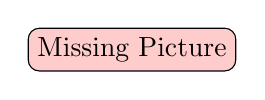
\begin{tikzpicture}
\draw(2,2) node [fill=red!20,draw,rounded corners]{Missing Picture};
\end{tikzpicture}
\end{center}
\end{wrapfigure} 
kind, called also \textit{trochoid} . It is generated in the following If the circle CDH roll on the given strait line AB, so that all the parts of the circumference be applied to it one after another, the point C that first touched the line AB in A, by a motion thus compounded of a circular and rectilinear motion, will describe the curve ACB, called the \textit{Cycloid}. 

\textbf{CYLINDER}. In geometry, a solid body, in form of a rolling stone, supposed to be generated by the rotation of a parallelogram about one of its sides.

\textbf{DAGGER}. A piece of timber that faces on to the poppets of the bilgeways, and crosses them diagonally, to keep them together. The plank that secures the heads of the poppets is called the \textit{Dagger Plank}. The word Dagger seems to apply to any thing that stands diagonally or aslant. \textit{See Frigate and Launch, Plate 9}. 

\textbf{DAGGER-KNEES}. Knees to supply the place of hanging knees. Their side arms are brought up aslant or nearly to the underside of the beams adjoining. They are chiefly used to the lower deck beams of merchant ships, in order to preserve as much stowage in the hold as possible. Any strait hanging knees not perpendicular to the side of the beam are in general termed \textit{Dagger-Knees}. 

\textbf{DAGGER-PLANK}. \textit{See} \textsc{Dagger}, above. 

\textbf{DATA}, in mathematics, are such things or quantities as are given or known, or assumed as known, in order to find thereby other things that are unknown. 

\textbf{DAVIT}. A short beam of fir, trimmed eight square towards the outer-end, and used as a crane, whereby the flukes of the anchor are hoisted to the Gunwale without injuring the planks of the side. 

\textbf{DEAD-DOORS}. Doors made of whole deal, with a slit deal lining, fitted in a rabbet to the outside of the gallery doors, and bolted within side, to prevent the water from flowing into the ship in case the quarter gallery should be carried away. 

\textbf{DEAD-EYES}. Oblate pieces of elm, fixed at the outer edges of the Channels, with three holes in each of them, through which the laniards of the shrouds are reeved. \textit{See Sheer Draught, Plate 1, and Sections, Plate 8}. 

\textbf{DEAD-FLAT}. A name given to that timber or frame which has the greatest breadth and capacity in the ship, and which is generally called the \textit{Midship Bend} i. In those ships where there are several frames or timbers of equal breadth or capacity, that which is in the middle should be always considered as Dead-Flat , and distinguished as such by this character $\bigoplus$. The timbers before Dead-Flat are marked A, B, C, \&c. in order; and those abaft Dead-Flat by the figures 1,2,3, \&c. The Timbers adjacent to Dead-Flat, and of the same dimensions nearly, are distinguished by the characters (A) (B) \&c. and (1) (2) \&c. \textit{See Sheer Draught, Plate 1}.

\textbf{DEAD-LIGHTS}. Shutters for the stern and gallery lights, to prevent the water from gushing into the ship in a high sea. They are made of whole deal, with slit deal linings, fitted on the outside, and bolted or otherwise fastened within, in bad weather.

\textbf{DEAD-RISING}, or \textsc{Rising Line} of the \textsc{Floor}. Those parts of the floor or bottom, throughout the ship's length, where the sweep or curve at the head of the floor timber is terminated or inflects to join the keel. Hence, although the rising of the floor at the midship-flat is but a few inches above the keel at that place, its height forward and aft increases according to the sharpness of form in the body. Therefore the rising of the floor in the \textit{sheer plan}, is a curve line drawn at the height of the ends of the floor timbers; and limited at the main frame, or dead-flat by the dead rising: appearing in flat ships nearly parallel to the keel for some timbers afore and abaft the midship frame; for which reason these timbers are called \textit{flats}: but in sharp ships it rises gradually from the main frame, and ends on the stem and post. 

\textbf{DEAD-WATER}. The eddy water which the ship draws after her at her seat or line of floatation in the water, particularly close aft. To this particular great attention should be paid in the construction of a vessel, especially in those with square tucks, for such being carried too low in the water, will be attended with great eddies or much dead-water. Vessels with a round buttock have but little or no \textit{dead-water}, because, by the rounding or arching of such vessels abaft, the water more easily recovers its state of rest. \textit{See the following Chapter on the Action of Fluids}. \&c.

\textbf{DEAD-WOOD}. That part of the basis of a ship's body, forward and aft, which is formed by solid pieces of timber scarfed together lengthwise on the keel. These should be sufficiently broad to admit of a stepping or rabbet for the heels of the timbers, that the latter not be continued downwards to sharp edges; and they should be sufficiently high to seat the floors. Afore and abaft the floors the dead-wood is continued to the cutting down line, for the purpose of securing the heels of the Cant-timbers. \textit{See Sheer Draught, Plate 1}. 

\textbf{DEAD WORK}. See \textsc{Supernatant}. 

\textbf{DEALS}. Fir Wood, of similar thickness to Plank. 

\textbf{DECKS}. The Decks are in a ship what floors are in a house. They are to support the may artillery, stores, \&c, and, with the beams, to connect the ship together. Their names arise from their situation, as \textit{Lower-Deck} , \textit{Middle-Deck}, \textit{Upper-Deck}, and \textit{Quarter-Deck}. When a deck stretches fore and aft upon one line, without any falls or intervals, it is called a \textit{Flush-Deck}. The space before the fore-most bulkhead, under the Quarter-Deck, is often called the\textit{ Half-Deck}; and, in some North Country ships, the steerage is frequently called by this name. \textit{See Plans of the Decks, Plates 5 and 6}. 

\textbf{DEEP-WAISTED}. A term signifying that the height of the topsides is much above the upper deck as they are in most vessels in the Royal Navy. 

\textbf{DEPTH in the} \textsc{Hold}. The height between the floor and the lower deck. This is one of the principal dimensions given for the construction of a ship. It varies according to the height at which the guns are required to be carried from the water; or, according to the trade for which a vessel is designed. 

\textbf{DIAGONAL LINE}. A line cutting the body-plan diagonally from the timbers to the middle line. It is square with, or perpendicular to, the shape of the timbers, or nearly so, till it meets the Middle Line. \textit{See Body Plan, Plate 1}. 

\textbf{DIAGONAL RIBBAND}. A narrow plank, made to a line formed on the Half-breadthplan, by taking the intersections of the diagonal line with the timbers in the body-plan to where it cuts the middle line in its direction, and applying it to their respective stations on the Halfbreadth-plan, which forms a curve to which the ribband is made as far as the Cant Body extends, and the square frame adjoining.\textit{ See Ribbands. See also the Frontispiece}. 

\textbf{DISPOSITION}. A draught or drawing representing the several timbers that compose the frame of the ship, so that they may be properly disposed with respect to the ports , \&c. \textit{See Disposition of the Frame, Plate 2}. 

\textbf{DOG}. An iron implement used by shipwrights, having a fang at one, or sometimes at each, end, to be driven into any piece for supporting it while hewing, \&c. Another sort has a fang in one end and an eye in the other, in which a rope may be fastened, and used to haul any thing along 

\textbf{DOG SHORE}. A Shore particularly used in Launching. \textit{See Frigate and Launch, Plate 9}.

\textbf{DOUBLING}. Planking of ships' bottoms twice. It is sometimes done to new ships when the original planking is thought to be too thin; and, in repairs, it strengthens the ship, without driving out the former fastenings. 

\textbf{DOVE-TAIL}. A score at the end of a piece of wood resembling the end of a dove's tail, and into which a corresponding piece is fitted. It is cut larger within than without for the purpose of holding the two pieces together the more firmly. See Half Breadth Plan of the Cutter , Plate 14. 

\textbf{DOVE-TAIL PLATES}. Metal plates, formed like Dove-tails, and used to confine the heel of the stern-post and keel together. \textit{See Frigate and Launch, Plate 9}. 

\textbf{DOWSING CHOCKS}. Pieces fayed athwart the Apron and lapped on the Knight-heads 

\textbf{DRAUGHT}. The drawing or design of the ship, upon paper, describing the different parts, and from which the ship is to be built. It is mostly drawn by a scale of one quarter of an inch to a foot, so divided or graduated that the dimensions may be taken to one inch. \textit{See Sheer Draught, Plate 1}. 

\textbf{DRAUGHT} \textsc{Of} \textbf{WATER}. The Depth of water a ship displaces when she is afloat. \textit{See Sheer Draught, Plate 1}. 

\textbf{DROP}. The fall or declivity of a deck, which is generally of several inches. Drops are also small foliages of carved work in the stern-munions, \&c. 

\textbf{DRIFT-PIECES}. Solid pieces, fitted at the drifts, to form the scroles. They are commonly mitered into the gunwale, but should rather be let in with square butts, as the caulking will stand better. \textit{See Sheer Draught, Plate 1}. 

\textbf{DRIFTS}. Those parts where the sheer is raised according to the heights of the decks or gangways, and where the rails are cut off and ended by scroles. S\textit{ee Sheer Draught, Plate 1}. 

\textbf{DRIVER}. The foremost spur on the bilgeways; the heel of which is fayed to the foreside of the foremost poppet, and cleated on the bulgeways, and the sides of it stand fore and aft. It is now seldom used. 

\textbf{DRUMHEAD}. The head of a capstan, formed of semi-circular pieces of elm, which, framed together, form the circle into which the capstan-bars are fixed. \textit{See Capstan, Plate 7}. 

\textbf{DRUXEY}. A state of decay in timber with white spungy veins, the most deceptive of any defect. 

\textbf{DUBBING}. Working with an adze.

\textbf{DUMB PINTLE}. See \textsc{Pintle}. 

\textbf{DUNNAGE-BATTENS}. Pieces of oak or fir, about two inches square, nailed athwart the flat of the orlop, to prevent wet from damaging the cables, and to admit air. Dunnage battens are also used in Sail-rooms, and in Magazines, so as to form a vacant space beneath the sails and powder barrels. \textsc{Dunnage}, in general, signifies light wood, or similar materials, used to elevate the stowage. 

\textbf{EARS} of \textsc{Boats}. The knee-pieces at the fore-part on the outside, at the height of the Gunwale. \textit{See Launch, Plate 25}. 

\textbf{EDGING of PLANK}. Sawing or hewing it narrower. 

\textbf{EKEING}. Making good a deficiency in the length of any piece by scarphing or butting, as at the end of deck-hooks, cheeks, or knees. The Ekeing at the lower part of the Supporter under the Cathead, is only to continue the shape and fashion of that part, being of no other service. We make this remark because, if the Supporter were stopt short without an ekeing, it would be better, as it causes the side to rot, and it commonly appears fair to the eye in but one direction. The Ekeing is also the piece of carved work under the lower part of the Quarterpiece at the aft part of the Quarter-gallery. \textit{See Sheer Draught, Plate 1, and Plans, Plates 5 and 6}. 

\textbf{ELEVATION}. The orthographic draught, or perpendicular plan of a ship, whereon the heights and lengths are expressed. It is called by shipwrights the \textsc{Sheer-Draught}. \textit{See Plate 1}. 

\textbf{ELLIPSIS} or \textsc{Ellipse}. A curve returning into itself, and produced by the section of a Cone by a plane cutting both its sides, but not parallel to its base. S\textit{ee Conic SECTIONS}. 

\textbf{ELLIPTIC} or \textbf{ELLIPTICAL}. Belonging to, or having some property of the Ellipsis. 

\textbf{ELLIPTICAL COMPASSES}. A mathematical instrument or machine for describing with facility the figure of an ellipsis. 

\textbf{ENTRANCE}. A term applied to the fore part of the ship under the load-water line; as, "She has a fine entrance," \&c. 

\textbf{EPICYCLOID}. In geometry, a curve generated by the revolution of a point of the periphery of a circle, by its rolling along the convex or concave side of the periphery of another circle, in the same manner that the Cycloid is described by the motion of a circle on a strait line. \textit{See Cycloid}. 

\textbf{EVEN KEEL}. A ship is said to swim on an even keel when she draws the same quantity of water abaft as forwards. 

\textbf{EYE-BOLT}. See\textsc{ Bolts}. 

\textbf{FACE-PIECE}. A piece of elm, generally tabled on to the fore part of the Knee of the Head, to assist the conversion of the main piece, and likewise to shorten the upper bolts, and prevent the cables from rubbing against them as the knee gets worn. \textit{See Sloop of War, Plate 10}. 

\textbf{FACING}. Letting one piece, about an inch in thickness, on to another, in order to strengthen it. 

\textbf{FAIR}. A term to denote the evenness or regularity of a curve or line. 

\textbf{FALL}. The descent of a deck from a fair curve lengthwise, as frequently in the upper deck of yachts, or merchant ships, to give height to the commander's cabin, and sometimes forward at the hawse-holes. 

\textbf{FALLING-HOME}, or, by some, \textsc{Tumbling-Home}. The inclination which the topside has within from a perpendicular. \textit{See} \textsc{Flairing}. 

\textbf{FALSE-KEEL}. A second keel, composed of elm-plank, or thick stuff, fastened in a slight manner under the main keel, to prevent it from being rubbed. Its advantages also are, that, if the ship should strike the ground, the false keel will give way, and thus the main keel will be saved; and it will be the means of causing the ship to hold the wind better. S\textit{ee Sheer Draught, Plate 1}. 

FALSE-POST\textbf{. A piece tabled on to the aft part of the heel of the main part of the stern post. It }is to assist the conversion and preserve the main post should the ship tail aground. \textit{See Sheer Draught, Plate 1}. 

\textbf{FALSE-RAIL}. A rail fayed down upon the upper side of the main, or upper rail of the head. It is to strengthen the head-rail, and forms the seat of ease at the after end next the bow. 

\textbf{FASHION PIECES}. The timbers so called from their fashioning the after part of the ship in the plane of projection, by terminating the breadth and forming the shape of the stern. They are united to the ends of the transoms and to the dead-wood. \textit{See Sheer Draught, Plate 1, and Laying-off, Plate 4}. 

To \textbf{FAY}. To join one piece so close to another that there shall be no perceptible space between them. 

\textbf{FENDERS}. Two pieces of oak plank fayed edgeways, perpendicularly, against the topsides abreast the main hatchway, to prevent the sides of the ship from being rubbed by the hoisting of any thing on board. It appears, however, from the construction of these Fenders, that their only use, in the Royal Navy, can be, when any thing is to be parbuckled up the side; and, as this is very uncustomary, most weights being hoisted on board by the yard-tackles, or a derrick, so that the articles never touch the sides, they are of little use, and had better be dispensed with, as they are the means of rotting the sides in the parts on which they are affixed. \textit{See Sheer Draught, Plate 1}. 

\textbf{FIFE-RAIL}. A rail formerly let over the timber heads above the Plank-sheers of the quarterdeck and forecastle, and formerly worked similar to the plank-sheer, but lately planked up to it, excepting the Taffarel Fife Rail. \textit{See Stern, Plate 1}. 

\textbf{FIGURE}. The principal piece of carved work or ornament at the head of the ship. \textit{See Sloop of War , Plate 10}. 

\textbf{FILAMENT} \textsc{of a stream}. See \textit{Stream}. 

\textbf{FILLING ROOM}. A small place in the Magazine, and lined with lead, and wherein the powder is started loosely to fill the cartridges. \textit{See Plans, Plate 5}. 

\textbf{FILLING-TIMBERS}. The intermediate timbers between the frames that are gotten up into their places singly after the frames are ribbanded and shored. \textit{See Disposition, Plate 2}. 

\textbf{FILLINGS}. Pieces of fir fayed between the cheeks of the Head ; and the pieces in general, to which no particular denomination is otherwise given, applied or affixed wherever solidity is required : such as those, of oak, between the floors to which the kelson is fayed; and, between the timbers, to receive the chain and preventer bolts, \&c. 

\textbf{FINISHINGS}. The carved ornaments of the Quarter Galleries. Those below the lower stool are called the Lower-finishings; and those above the upper stool, the Upper-finishings. \textit{See Sheer Draught, Plate 1}. 

\textbf{FIRE HEARTH}. The fire-place and conveniencies in the Gallery for cooking the provisions for the people. It is composed of a grate, iron-boilers, ovens, a smoke-jack, \&c. 

\textbf{FISH-ROOM}. A place parted off in the after-hold, by bulkheads, between the Spirit-Room, Bread-Room, and Powder-Room. It was formerly used for stowing the salt-fish to be consumed on board, a practice long since discontinued. It is now used for the stowage of coals, and sometimes for spirits, when the ship is destined for a long voyage. \textit{See Inboard Works, Plate 4}. 

\textbf{FIXED-BLOCKS}. Those blocks that come through the sides and are bolted, as the Sheet, Tack, and Brace, Blocks. \textit{See} \textsc{Blocks}. \textit{See also Disposition of the Frame, Plate 2}. 

\textbf{FLAIRING}. The reverse of \textit{Falling} or \textit{Tumbling-Home}. As this can be only in the forepart of the ship, it is said that a ship has a \textit{flairing-bow} , when the topside falls outward from a perpendicular. Its uses are, to shorten the Cathead, and yet keep the anchor clear of the bow. It also prevents the sea from breaking in upon the Forecastle, \textit{See the Sloop of War, Plate 10}.

\textbf{FLATS}. A name given to the timbers a-midships that have no bevellings, and are similar to dead-flat, which is distinguished by this character $\oplus$. \textit{See} \textsc{Dead-flat}. \textit{See also Sheer Draught, Plate 1}. 

\textbf{FLEXURE}. The bending or curving of a line or figure. \textit{See} \textsc{Inflected Curves}. 

\textbf{FLIGHT}. A sudden rising, or a greater curve than sheer, as the cheeks, Catheads, \&c.

\textbf{FLIGHT} of the \textbf{TRANSOMS}. As the ends or arms of the transoms, being gradually closed in proportion to their distance from the Wing transom, downwards, become more narrow as they approach the keel, the general figure or curve which they thus describe, similar to the rising of the Floors, is called the \textit{Flight of the Transoms}. 

\textbf{FLOOR}. The bottom of a ship, or all that part on each side of the keel which approaches nearer to a horizontal than a perpendicular direction, and whereon the ship rests when aground. 

\textbf{FLOOR-HOLLOW}. The inflected curve that terminates the floor next the keel, and to which the \textit{floor hollow mould} is made. \textit{See Moulds, Plate 1 of Laying-off}. 

\textbf{FLOOR-RIBBAND}. The ribband next below the floor-heads which supports the floors. This ribband should be well shored, and great pains should be taken to keep it fair and level, as the whole fabric depends very much thereon. \textit{See Plate 1, of Laying-off}. 

\textbf{FLOOR SWEEPS}. The Radii that sweep the heads of the Floors. See \textsc{Frames}. \textit{See also Sheer Draught and Body Plan, Plate 1}. 

\textbf{FLOORS}, or \textsc{Floor Timbers}. The timbers that are fixed athwart the keel, and upon which the whole frame is erected. They generally extend as far forward as the fore-mast, and as far aft as the after square timber; and, sometimes, one or two cant-floors are added. \textit{See} \textsc{Frames}. \textit{See also Midship Sections, Plate 8}. 

\textbf{FLUSH}. With a continued even surface: As A \textit{flush deck}, which is a deck upon one continued line, without interruption, from fore to aft.

\textbf{FOCUS}, in geometry and conic sections. Certain points in the parabola, ellipsis, and hyperbola, where the rays reflected from all parts of these curves concur and meet. See \textsc{Conic Sections}. 

The \textsc{Foci} of an \textsc{Ellipsis} are two points in the longest axis, from which, as centres, the figure. is described. If from the Foci two right lines be drawn, meeting each other in the periphery of the ellipsis, their sum will be equal to the longest axis; and therefore when an ellipsis and its two axis are given, and the foci are required, you need only take half the longest axis with compasses, and setting one foot in the end of the shorter, the other foot will cut the longer in the focus required. 

The \textsc{Focus} of an \textsc{Hyperbola} is that point in the axis through which the \textit{latus rectum} passes; when, if any two right lines are drawn meeting in either of the opposite hyperbolas, their difference will be equal to the principal axis. 

The \textsc{Focus} of \textsc{a parabola}, is a point in the axis within the figure, distant from the vertex one fourth part of the \textit{latus rectum}. 

\textbf{FOOT SPACE RAI}L. The rail that terminates the foot of the balcony, and in which the ballasters step, if there be no Pedestal Rail. It rabbets over the ends of the deals of the deck. \textit{See Sheer Draught and Perpendicular View of the Stern, Plate 1}. 

\textbf{FOOT-WALING}, or Futtling, or Ceiling. The inside plank of the ship's bottom. \textit{See Midship Sections, Plate. 8}. 

\textbf{FORE}. The distinguishing character of all that part of a ship’s frame and materials which lie toward the sterm.

\textbf{FORE and AFT}. In the direction of the ship's length from head to stern. 

\textbf{FORE BODY}. That part of the ship’s body, afore the Midships or Dead-flat. See Bodies. This term is more particularly used in expressing the figure or shape of that part of the ship. \textit{See Body Plan, Plate 1}. 

\textbf{FORE-CASTLE}. The short deck above the upper deck forward. \textit{See Plans, Plate 6}. 

\textbf{FORE-FOOT}. The foremost piece of the Keel. \textit{See Sheer Draught, Plate 1}. 

\textbf{FORE-LOCK}. A thin circular wedge of iron, used to retain a bolt in its place, by being thrust through a mortise hole at the point of the bolt. It is sometimes turned or twisted round the bolt to prevent its drawing. FORE-MOST. Nearest to the head of the ship. 

\textit{FORE PEEK}. Close forward under the lower deck. \textit{See Inboard Works, Plate 4, and Plans, Plate 5}. 

\textbf{FORK-BEAM}. See \textsc{Beams}. 

\textbf{FORWARD}. In the fore-part of the ship. 

\textbf{FRAMES}. The bends of timber which form the body of the ship; each of which is composed of one \textit{floor-timber}, two or three futtocks , and a \textit{top-timber} on each side; which, being united together, forın the frame. Of these frames, or bends, that which incloses the greatest space is called the \textit{midship} or \textit{main frame} or \textit{bend}. The arms of the floor timber form a very obtuse angle ; and in the other frames, this angle decreases or gradually becomes sharper, fore and aft, with the middle line of the ship. Those floors which form the acute angles afore and abaft are called the Rising Floors. \textit{See Body Plan, Plate 1, and Midship Sections, Plate 8. }

A frame of timbers is commonly formed by arches of circles called \textit{Sweeps}, of which there are generally five: 1st. The \textit{Floor Sweep}, which is limited by a line in the Body Plan perpendicular to the plane of elevation, a little above the keel; and the height of this line above the keel is called the \textit{Dead Rising}. The upper part of this arch forms the head of the floor timber. 2nd. The \textit{Lower Breadth Sweep}; the centre of which is in the line representing the lower height of breadth. 3rd. \textit{The Reconciling Sweep}; this sweep joins the two former, without intersecting either; and makes a fair curve from the lower height of breadth to the rising line. If a straight line be drawn from the upper edge of the keel to touch the back of the floor sweep, the form of the midship frame below the lower height of breadth will be obtained. 4th. The \textit{Upper Breadth Sweep}; the centre of which is in the line representing the upper height of breadth of the timber. This sweep described upwards forms the lower part of the top timber. 5th. \textit{The Top-Timber Sweep}, or \textit{Back Sweep}, is that which forms the hollow of the top-timber. This hollow is, however, very often formed by a mould, so placed as to touch the upper breadth sweep, and pass through the point limiting the half-breadth of the top-timber. \textit{See Disposition of the Frame , Plate 2. See also the Frontispiece}. 

\textbf{FRAME TIMBERS}. The various timbers that compose a frame bend; as the floor timber, the first, second, third, and fourth, futtocks, and top timber, which are united, by a proper shift, to each other, and bolted through each shift. They are often kept open, for the advantage of the air, and fillings fayed between them in wake of the bolts. Some ships are composed of frames only, and are supposed to be of equal strength with others of larger scantling. \textit{See Disposition, Plate 2. See also Midship Sections, Plate 8}. 

\textbf{FRIEZING}. The ornamental carving or painting above the drift-rails, and likewise round the stern or bow. It is generally a representation of foliage or emblematic trophies of war, \&c. FULCRUM. The prop of support of a lever in lifting or moving a heavy body. 

\textbf{FURRENS}. Pieces to supply the deficiency of timber the moulding way. 

\textbf{FUTTLING}. \textit{See} \textsc{Footwaling}. 

\textbf{FUTTOCKS}. The separate pieces of timber of which the frame timbers are composed. They are named according to their situation, that nearest the keel being called the first futtock, the next above, the second futtock, \&c. \textit{See} \textsc{Frames}. \textit{See also Midship Sections, Plate 8}. 

\textbf{GALLERY}. The long narrow compartment, or balcony, projecting from the stern and quarters of a large ship. The Stern gallery is usually decorated with a ballustrade. \textit{See} \textsc{Quarter Galleries}. \textit{See also Sheer Draught, Plate 1}. 

\textbf{GALLEY}. The place appointed for the fire-hearth and the use of the cooks. It is generally under the Forecastle or the fore part of the ship. \textit{See Plan of Upper Deck, Plate 6}. 

\textbf{GAMMONING-HOLE}. A mortise hole cut through the knee of the head, between the cheeks, through which the rope passes that gammons the bowsprit. \textit{See Sloop of War, Plate 10.} 

\textbf{GANGBOARDS}. The narrow platforms within the sides, next the Gunwales, which connect the quarter deck to the forecastle. Each is composed of three or four Prussia deals fayed and bolted together edgewise. \textit{See Plan of Quarter Deck and Forecastle , Plate 6}. 

\textbf{GANGWAY}. The entrance into the ship by the steps on the side, which, of course, is best when flush with the quarter-deck. \textit{See Sheer Draught , Plate 1 , and Plan of Quarter Deck and Forecastle , Plate 6}. 

\textsc{A Fixt Gangway} is a continuation of the quarter-deck to a knee before it, so as to form the gangway when the quarter-deck of itself reaches not forward enough. There is sometimes a fixed gangway, made at the aft part of the forecastle in large ships, when the waist is longer than the customary length of a deal. S\textit{ee Plan of Quarter-Deck and Forecastle, Plate 6}. 

\textbf{GARLANDS}. See \textsc{Shot-Garlands}. 

\textbf{GARBOARD STRAKE}. That strake of the bottom which is wrought next the keel, and rabbets therein. \textit{See Planking, Plate 3}. 

\textbf{GENESIS}, among mathematicians, signifies the formation or production of some figure or quantity. 

\textbf{GENERATING LINE}, or \textsc{Figure}, in Geometry, is that line, which by its motion produces F any plane or solid figure. Thus a right line moved any way parallel to itself generates a parallelogram; moved round a point in the same plane with one end fastened in that point, it generates a circle. One entire revolution of a circle, in the same plane, generates the cycloid ; and the revolution of a semi-circle round its diameter generates a sphere. See \textsc{Cycloid} and \textsc{Sphere}. 

\textbf{GOOGINGS} or \textsc{Gudgeons}. The hinges upon which the rudder traverses. \textit{See Rudder, in Sheer Draught, Plate 1}. Also the the metal pieces upon which a windlass works. 

\textbf{GOOSE-NECK}. A large iron hook fixed with a strap at the after end of the main channel to stow the studding-sail boom in. 

A \textsc{shifting goose neck} is a sort of iron cleat confined near the foremost end of the Tiller by means of thin iron plates, one on each side, which are bolted through the tiller, so that the gooseneck may move forward between the plates as in a grove. Its use is to shift forward as the tiller may shrink and go aft, to be kept fast in the rudder. The goose-neck is fastened by two screw eye-bolts, which go through it, and jamb it upon the tiller. \textit{See} the Tiller and Gooseneck in the \textit{Inboard Works, Plate 4, and Upper Deck Plan, Plate 6}. 

\textbf{GRAIN-CUT}. Cut athwart the grain; as when the grain of the wood does not partake of the shape required. For instance, if a knee be cut out of a broad straight grained plank, it is evident that the grain being cut across, would be very short in one or both the arms. 

\textbf{GRATINGS}. The lattice coverings of the hatchways, which are made with openings to admit air, or light, by cross battens and ledges. The openings should never be so large as to admit the heel of a man's shoe, as they may otherwise endanger those who pass over them. 

\textbf{GRAVITY}. That quality by which bodies naturally tend downwards and towards a centre.

Gravity may be considered as a property of matter, which, although not essential, is universal; and, in one sense, inseparable from it. That is, all matter, however modified, and all bodies, have a gravitation or attraction towards each other. 

All bodies on or near the Earth have a gravity, or weight, or a tendency towards its centre, or at least perpendicular to its surface; and this law is found universally to hold with respect to all known bodies and matter in nature. It is therefore acknowledged as a principle or law of nature, that all bodies, and all the particles of all bodies, mutually gravitate towards each other. 

Bodies immersed in fluids have two kinds of gravity, the one \textit{absolute} and the other \textit{relative}. By the former is meant the whole force wherewith a body tends downwards ; and, by the latter, the excess of gravity whereby a body tends downwards more than the fluids which surround it. 

\textsc{Specific Gravity}, called also relative, comparative, and apparent gravity, is that by which one body is said to be heavier or lighter than another of a different kind. Thus lead is said to be specifically heavier than cork; because, supposing an equal bulk of each, the one would be heavier than the other. 

Hence it follows, that a body specifically heavier than another is also more dense; that is, contains a greater quantity of matter under the same bulk, because bodies weigh in proportion to the quantity of matter they contain. 

If a solid be immersed in a fluid of the same specific gravity with itself, it will remain suspended therein, in whatever part of the fluid it is placed : but, if the body immersed is specifically heavier than the fluid, it will subside to the bottom. On the contrary, if the body is specifically lighter than the fluid, it will rise to the top. 

A body being laid on the surface of a fluid specifically heavier than itself sinks in it till the immersed part has displaced a quantity of fluid whose weight is equal to that of the whole body: and a body suspended in a fluid specifically lighter than itself loses a part of its weight equal to that of the fluid of the same bulk. \textit{See} \textsc{Specific Gravity}. 

\textbf{GRIPE}, A piece of elm timber that completes the lower part of the knee of the head, and makes a finish with the fore-foot. It bolts to the stem, and is farther secured by two plates of copper in form of a horse-shoe, and therefrom called by that name. See \textit{Sheer Draught, Plate 1}.

\textbf{GROMMETS} \textsc{for Boats}. Wreaths of rope which confine the oars to the pins in the Gunwale.

\textbf{GROUNDWAYS}. Large pieces of timber, generally defective, which are laid upon piles driven in the ground, across the dock or slip, in order to make a good foundation to lay the blocks on, upon which the ship is to 'rest. 

\textbf{GUARD-IRONS}. Carved or arched bars of iron fixed over the carved work of Yachts, \&c particularly over the head and quarter pieces, to prevent their being damaged. 

\textbf{GUNNER's STORE-ROOM}. \textit{See} \textsc{Store-Rooms}. 

\textbf{GUN-ROOM}. The after part of the lower deck, parted off for the accommodation of the subaltern officers. \textit{See Plans, Plate 5}. 

\textbf{GUNWALE}. That horizontal plank which covers the heads of the timbers between the main and fore drifts. S\textit{ee Sheer Draught , Plate 1}. 

\textbf{GUY}. A rope extended from the head of sheers, and made fast at a distance on each side, by which they are kept steady. 

\textbf{HAIR BRACKET}. The moulding which terminates the fore ends of the head rails, comes at the back of the figure, and breaks in fair with the upper cheek. \textit{See Sheer Draught , Plate 1}. 

\textbf{HALF-BREADTH PLAN}. \textit{See} \textsc{Plan}. 

\textbf{HALF-BREADTH} \textsc{of the} \textbf{RISING}. A curve in the Floor plan, which limits the distances of the centres of the floor sweeps from the middle line of the body plan. \textit{See Half-Breadth Plan, Plate 1}. 

\textbf{HALF-PORTS}. A sort of shutters made of deal, and fitted to the stops of those ports which have no hanging lids. They have a hole cut in them for the gun to go through. 

\textbf{HALF-TIMBERS}. The short timbers in the cant bodies which are answerable to the lower futtocks in the square body. \textit{See Disposition, Plate 2}. 

\textbf{HAMMACOE} or \textbf{HAMMOCK RACKS}. The battens nailed to the sides of the beams, and to which the sailors hang their hammocks and bedding. 

\textbf{HAMMERS}. The tools used by shipwrights for driving nails and drawing bolts. \textit{Claw Hammers} are the most convenient for the former purpose, having a claw at one end to draw the nail out if it'splits or rucks in driving. \textit{Clench Hammers} should be made of hard steel, with one flat end for clenching, and a face for smoothing the clench. 

\textbf{HANCE} or \textbf{HANCH}. A sudden fall or break, as from the drifts forward and aft to the waist. Also those breaks in the rudder, \&c. at those parts where it suddenly becomes narrower. \textit{See Sheer Draught, Plate 1}. 

\textbf{HANDSPEC}. A wooden bar, made of tough ash, and used as a lever to prize or remove great weights. 

\begin{wrapfigure}{r}{0.15\textwidth}
\begin{center}
\includegraphics[scale=0.5]{pictures/hand_screw}
\end{center}
\end{wrapfigure} \textbf{HAND SCREWS} or \textbf{JACKS}, double or single. The Engine  represented in the margin, used to cant beams or other weighty timbers. It consists of a box of elm, containing cogged iron wheels, of increasing powers. The outer one, which moves the rest, is put in motion by a winch on the outside, and is called either single or double, according to its increasing force. The outer figure here shewn represents the inside work separately. 

\textbf{HANGING}. Declining in the middle part from a horizontal right line, as the hanging of the decks, hanging of the sheer, \&c. 

\textbf{HANGING-CLAMP.} A semi-circular iron, with a foot at each end, to receive nails, by which it is fixed to any part of a ship, to hang stages to, \&c. 

\textbf{HANGING-KNEE}. Those knees against the sides whose arms hang vertically or perpendicular. \textit{See Midship Sections, Plate 8}. 

\textbf{HARPINS}. Pieces of oak, similar to ribbands, but trimmed and bevelled to the shape of the body of the ship, and holding the fore and after cant bodies together until the ship is planked. But this term is mostly applicable to those at the bow; hence arises the phrase "clean and full harpin," as the ship at this part is more or less acute. \textit{See Plate 8 of Laying-off}. 

\textbf{HARRIS-CUT}. This term is applied when the edges of planks are cut to an under bevelling, to fay one on another, as the birthing or sides of the well, so that no ballast may get in at the joints. 

\textbf{HATCHES}. The covering for the Hatchways. 

\textbf{HATCHWAYS}. The Square or oblong openings in the middle of the decks, for the convenience of lowering down goods; forming also the passages from one deck to another and into the Hold, \&c. \textit{See Plans of Decks, Plates 5 and 6}. 

\textbf{HAWSE-HOOK}. The Breasthook over the Hawse-holes. See \textit{Inboard Works, Plate 4}. 

\textbf{HAWSE-PIECES}. The timbers which form the bow of the ship, whose sides stand fore and aft, or nearly so; that is, parallel to the middle line of the ship. \textit{See Disposition, Plate 2, and Plate 7 of Laying-off}. 

\textbf{HEAD}. The upper end of any thing; but more particularly applied to all the work fitted afore the stem, as the Figure, the Knee, Rails, \&c. \textit{See Sheer Draught, Plate 1}. 

\textsc{A Scroll Head} signifies that there is no carved or ornamental figure at the head, but that the termination is formed and finished off by a volute , or scroll turning outwards. 

\textsc{A Fiddle Head} signifies a similar kind of finish, but with the scroll turning aft or inwards. 

\textbf{HEAD-LEDGES}. The 'thwartship pieces which frame the hatchways and ladderways. \textit{See Plans, Plates 5 and 6}. 

\textbf{HEAD-RAILS}. Those rails in the Head which extend from the back of the figure to the cathead and bows, which are not only ornamental to the frame, but useful to that part of the ship. \textit{See Sheer Draught, Plate 1}. 

\textbf{HEAD-TIMBERS}. The pieces that cross the rails of the head vertically. They are bolted through their heels to the cutting-down of the knee, and unite the whole together. \textit{See Sheer Draught, Plate 1}. 

\textbf{HEEL}. The lower end of a tree, timber, \&c. A ship is also said to Heel when she is not upright but declines towards the stern. 

\textbf{HEIGHT of BREADTH LINES}, \textsc{Upper} and \textsc{Lower}. The two curved lines described on the Sheer-plan, at the height of the main breadth, or broadest part of the ship, at each timber. In the Body-plan, they are horizontal lines at those heights on which the Main-breadths of each timber are set off. In those lines are found the centres for sweeping the lower and upper breadth sweeps. \textit{See} \textsc{Main Breadth}. \textit{See also Sheer Draught, and Body-plan, Plate 1}. 

\textbf{HELM}. The whole of the machinery astern which serves to steer or guide the ship, as the rudder, the tiller, the wheel, \&c. \textit{See Inboard Works, Plate 4}. 

\textbf{HELM-PORT}. That hole through the counter, through which the head of the rudder passes. \textit{See Sheer Draught, Plate 1}. 

\textbf{HELM-PORT TRANSOM}. The piece of timber placed athwart the inside of the counter timbers at the height of the Helm-Port. It is bolted through every stern timber, and knee'd at each end for the security of that part of the ship. \textit{See Perpendicular View of the Stern,in Plate 1}. 

\textbf{HELVE}. The handle of axes, adzes, mauls, \&c. 

\textbf{HETEROGENEOUS} or \textsc{Heterogenal}. Any thing consisting of parts of dissimilar kinds, in opposition to \textit{Homogeneous} . In mechanics, it is expressive of bodies of unequal density in different parts of their bulk; or of such whose gravities in different parts are not proportionable to the bulk of the whole; whereas bodies equally dense or solid in every part, or whose gravity is proportionable to their bulks, are said to be \textit{homogeneous}. 

\textbf{HOGGING}. See \textbf{broken backed}. A ship is said to \textit{Hog} when the middle part of her keel and bottom are so strained as to curve or arch upwards. This term is therefore opposed to \textit{Sagging}, which, applied in a similar manner, means, by a different sort of strain, to curve downwards. 

\textbf{HOLD}. That part of the ship below the lower deck, between the bulkheads, which is reserved for the stowage of ballast, water, and provisions, in ships of war, and for that of the cargo in merchant-vessels. 

\textbf{HOLLOW-MOULD}: The same with \textit{Floor-Hollow}, which see. Sometimes the back sweep which forms the upper part of the top-timber is called the \textit{Top-timber Hollow}. \textit{See Moulds, Plate 1 of Laying-off}. 

\textbf{HOMOGENEOUS}. Of a like kind throughout, and having the same nature and properties. 

\textbf{HOOD}. The name given to all the foremost and aftermost planks of the bottom, both withinside and without. Also a covering to shelter the mortar in Bomb-vessels. In merchant ships it is the birthing round the ladder way. \textit{See} \textsc{Companion}. 

\textbf{HOODING ENDS}. Those ends of the planks which bury in the rabbets of the stem and stern post. 

\textbf{HOOK} of the \textsc{Decks}. See \textsc{Breast-Hooks}. 

\textbf{HOOKING}. The act of working the edge of one plank, \&c. into that of another, in such a manner that they cannot be drawn asunder endways. S\textit{ee Kelson Scarphs, Inboard Works, Plate 4, and Sheer Strakes, Planking, Plate 3}. 

\textbf{HORIZONTAL RIBBANDS}. Those ideal ribbands, used in laying off, which are taken off level or square with the middle line of the ship's body. \textit{See} \textsc{Ribbands}. 

\textbf{HORN} or \textbf{HORNING}. Placing or proving any thing to stand square from the middle line of the ship, by setting an equal distance thereon from each side of the middle line ; then bringing the same distances equally from some fixed spot in the middle line by a batten or staff of some length. 

\textbf{HORSE}. The round bar of iron which is fixed to the main rail and back of the figure in the Head, with stantions, and to which is attached a netting for the safety of the men who have occasion to be in the Head. Also the cross piece of timber tenoned on to the heads of the bitts for the booms to rest upon. 

\textbf{HORSE-IRON}. An iron fixed in a handle, and used with a beetle by caulkers, to \textit{horse-up} or harden in the oakum. 

\textbf{HORSE-SHOES}. Large straps of iron or copper shaped like a horse-shoe and let into the stem and gripe on opposite sides, through which they are bolted together to secure the gripe to the stem. 

\textbf{HULL}. The whole frame or body of a ship, exclusive of the masts, yards, sails, and rigging. 

\textbf{HYDROSTATICS}. That science which treats of the weight, pressures, motion, and equili-, bria, of fluids; and which ought, therefore, to be thoroughly understood by every shipwright desirous of possessing a competent knowledge of the theoretic principles of his art. 

\textsc{Hydraulics} is that part of Statics which considers the \textit{motion} of fluids, with the application thereof to machinery, and is distinguished from \textit{Hydrostatics} in this, that the latter is supposed merely to explain the equilibrium of fluids, or the gravitation of fluids at rest. From the immediate relation between the two, it however frequently happens, that they are considered as one, and indiscriminately denominated either \textit{Hydrostatics} or \textit{Hydraulics}. 

\textbf{HYPERBOLA}. A figure made by the section of a cone. See \textit{Conic Sections}.

\textbf{JAMBS} for fixing the Lights. Thick broad pieces of oak, fixed up endways, and between which the magazine lights are fitted. \textit{See Magazine Plan, Plate 5}. 

\textbf{IMPETUS}. The force with which one body strikes or impels another. 

To \textbf{IMPINGE}. To, dash or strike against; to clash with. 

\textbf{IMPULSION} \textsc{of a Fluid}. The influence or action of a fluid in motion on a solid body, as of a stream or current of water on that of a ship. 

\textsc{Direct Impulse} expresses the action of a particle, filament, or stream, of fluid, when meeting the surface perpendicularly, or when the surface is perpendicular to the direction of the stream. 

\textsc{Absolute Impulse} means the absolute pressure on the impelled surface, arising from the action of the fluid, whether striking the surface perpendicularly or obliquely; or, it is the force impressed on the surface, or tendency to motion which it acquires, and must be opposed by an equal force in the opposite direction, in order that the surface may be maintained in its place. This pressure is always perpendicular to the surface : it having been determined, by universal experience, that the mutual actions of bodies on each other are always exerted in a direction perpendicular to the touching surfaces; as, when one billiard ball is struck by another, moving in any direction whatever, the first ball always moves off in the direction perpendicular to the plane which touches the two balls in the point of contact or impulse. 

\begin{wrapfigure}{r}{0.25\textwidth}
\begin{center}
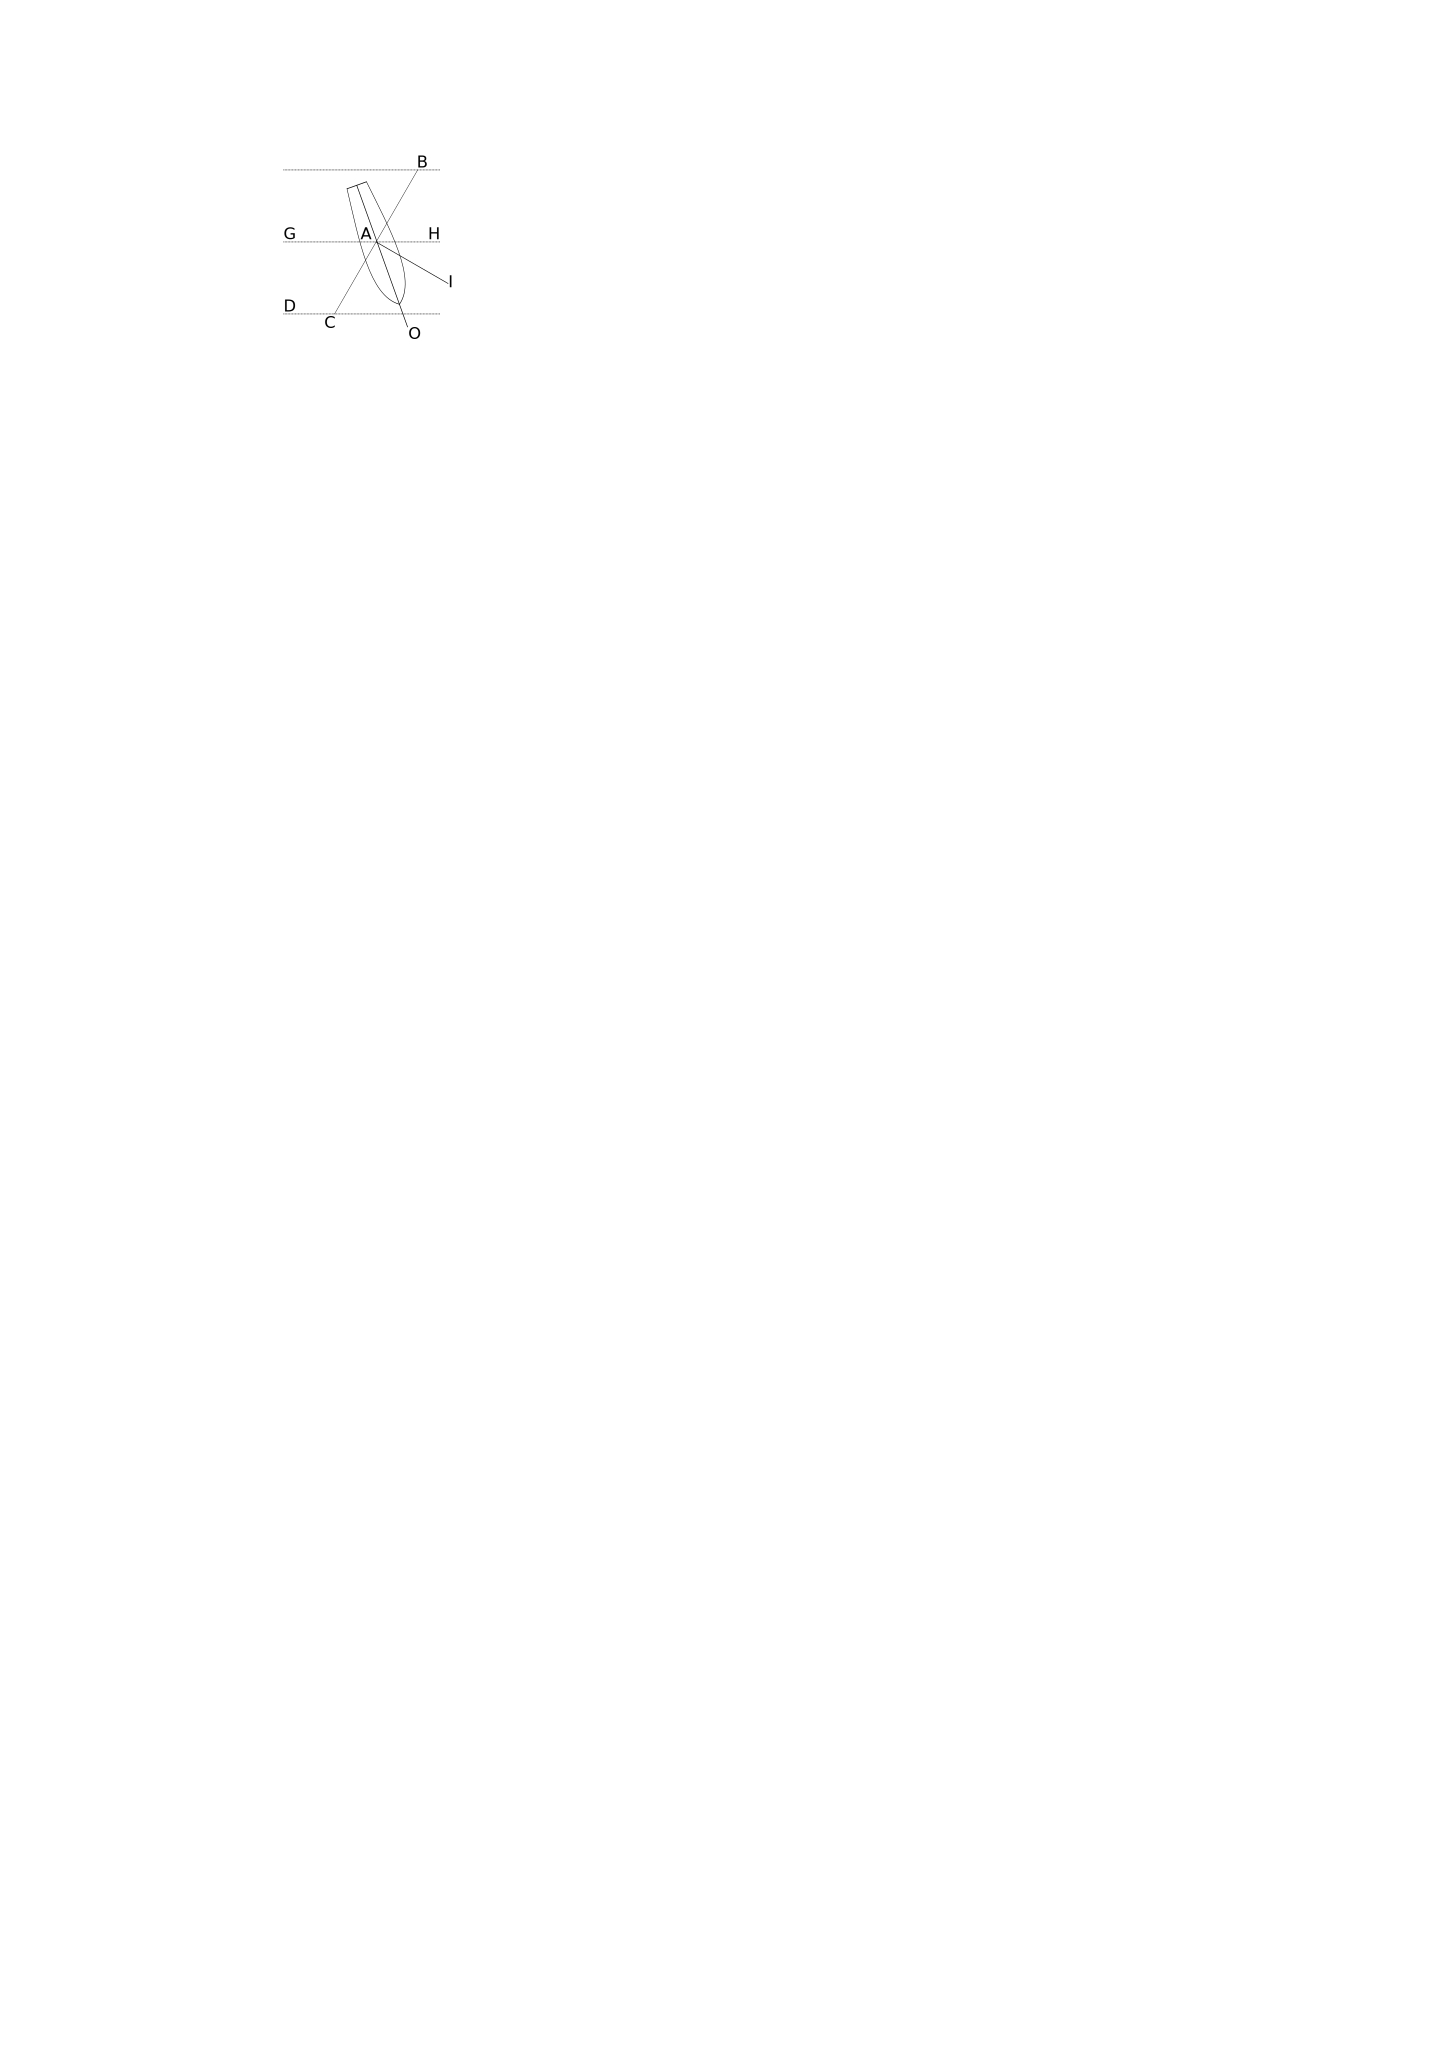
\includegraphics[trim=0cm 0cm 0cm 0cm, clip]{pictures/Impulsion}
\end{center}
\end{wrapfigure}
\textsc{Relative or effective Impulse} is the pressure on the surface estimated in some particular direction. Thus BC, in the annexed figure, may represent the sail of a ship, impelled by the wind blowing in the direction DC. A0 may be the direction of the ship's keel, or the line of her course. The wind strikes the sail in the direction GH parallel to DC; the sail is urged or pressed in the direction Al, perpendicular to BC. But we are interested to know what tendency this will give the ship to move in the direction AO; and this is the \textit{relative or effective impulse}. 

The \textsc{Angle of Incidence} of the wind (which has been already defined under the article ANGLE) is the angle contained between the direction of the wind GA and the plane BC. 

The \textsc{Angle of Obliquity} is the angle OAC contained between a plane, BC, and the direction AO, in which it may be required to estimate the impulsion of a fluid, \&c. which comes in the direction GA. 

\textbf{IN} \textsc{and} \textbf{OUT}. A term sometimes used for the scantling of the Timbers the moulding way, but more particularly applied to those bolts in the knees, riders, \&c. which are driven through the ship's sides, or athwartships, and therefore called "\textit{In and out Bolts}." 

\textbf{INBOARD}. Within the ship; as the \textit{Inboard Works}, \&c. \textit{See Plate 4}. 

\textbf{INCIDENCE}. The direction in which one body strikes or falls upon another. The angle made by \textit{See} \textsc{Angle}, \textit{and Fig. 2, Plate A}. 

\textbf{INCLINED PLANE}. A plane that makes an oblique angle with the horizon. 

\textbf{INFLECTED CURVES}. Such curves as have a point of inflection, and which, being continued, turn a contrary way; as the water lines abaft, of ships in general. 

\textbf{INNER POST}. A piece of oak timber, brought on and fayed to the foreside of the main sternpost, for the purpose of seating the Transoms upon it. It is a great security to the ends of the planks, as the main post is seldom sufficiently afore the rabbet for that purpose, and is also a great strengthener to that part of the ship. \textit{See Inboard Works, Plate 4}. 

\textbf{INTERSECTION}. The point in which one line crosses another. 

\textbf{JOINT}. The place where any two pieces are united. This term is, however, more particularly used to express the lines which are laid down in the mould-loft for the purpose of making the moulds for the timbers, as those lines exhibit the shape of the body between every two timbers, which is hence called the \textit{Joint}. 

\textbf{IRONS}. The tools used by the caulkers for driving in the oakum. 

\textbf{KEEL}. The main and lowest timber of a ship, extending longitudinally from the stem to the stern post. It is formed of several pieces, which are scarphed together endways, and form the basis of the whole structure. Of course it is usually the first thing laid down upon the blocks for the construction of the ship. \textit{See Sheer Draught , Plate 1}. 

\textbf{KEEL STAPLES}. See \textsc{Staples}. 

\textbf{KEELSON} or, more commonly, \textbf{KELSON}. The timber, formed of long square pieces of oak, fixed within the ship exactly over the keel, (and which may therefore be considered as the counter part of the latter) for binding and strengthening the lower part of the ship; for which purpose it is fitted to, and laid upon, the middle of the floor timbers, and bolted through the floors and keel. \textit{See Inboard Works, Plate 4}. 

\begin{wrapfigure}{r}{0.25\textwidth}
\begin{center}
\includegraphics[scale=0.5]{pictures/kevels}
\end{center}
\end{wrapfigure}
\textbf{KEVELS}. Pieces of oak plank, shaped like timber heads, and fixed into mortises cut through other pieces that are fastened to the insides of the ship. They answer the purpose of timber heads to belay ropes to. 

\textbf{KEVEL} or \textbf{CAVEL HEAD BLOCKS}. A Sort of Blocks, having a sheave hole or two, cut through fore and aft, and which are bolted to the ship's sides, nearly opposite the masts, to reeve the lifts, \&c. 

\textbf{KEY}. A dry piece of oak, \&c. cut tapering, to drive into scarphs that have hook-butts.

\textbf{KILN}. A convenience for heating planks to make them pliable. A Sleam - Kiln is a trunk composed of deals, grooved neatly into each other, which is generally from three to four feet square, and from forty to sixty feet in length, having a door at each end. It is confined together by bolts driven through it at certain distances, which answer for bearers to rest the plank upon, and it is supported upon brick-work. Beneath it, in the middle, is a large iron or copper boiler, or sometimes two boilers, which are then fixed near each end, the steam from which, issuing into the trunk, enters the pores of the plank and makes it pliable. 

A \textit{Boiler Kiln} is shaped similar to the former, but with an open top. It is formed of sheets of copper rivetted together, and is fixed in brick work. Under each end, or in the middle, are furnaces to make the water boil, when the plank is in. The upper part is covered with shutters that are hoisted occasionally by small tackles. The dimensions, \&c. of a copper boiler in one of the Royal Yards are, length, forty feet; breadth, at the ends, four feet three inches, and in the middle, six feet ; depth, two feet ten inches; and weight fifty-three cwt. three qrs. seven lb. 

KNEES. The crooked pieces of oak timber by which the ends of the beams are secured to the sides of the ship. Of these, such as are fayed vertically to the sides are called \textit{Hanging-Knees}, and such as are fixed parallel to, or with the hang of, the deck, are called \textit{Lodging-Knees} . \textit{See Midship Şections, Plate 8, and Plans of Gun-deck, Plate 5}. 

KNEE TIMBER. That sort of crooked timber which forms, at its back or elbow, an angle of from forty-five to twenty-four degrees, with a line produced or continued in the direction of one of its outer sides. If it forms the greater angle, it is the more valuable on that account. But if the angle so formed at the back be more acute, the wood is said to be \textit{raking} , and is proportionally less valuable, being of the less utility for the formation of knees, \&c. 

\textbf{KNEE of the HEAD}. The large flat timber fayed edgeways upon the fore-part of the stem. It is formed by an assemblage of pieces of oak coaked or tabled together edgewise, by reason of its breadth, and it projects the length of the Head. Its fore-part should form a handsome serpentine line, or inflected curve. The principal pieces are named the \textit{Main-piece} and \textit{Lacing}. \textit{See Sheer Draught, Plate 1}. 

\textbf{KNIGHT-HEADS}, or \textsc{Bollard Timbers}. Large oak timbers fayed and bolted to each side of the stem, the heads of which run up sufficiently above the head of the stem to support the bowsprit, care being taken to cast them-sufficiently open above the stem to the diameter of the bowsprit. \textit{See Sheer Draught, Plate 1}. 

\textbf{KNUCKLE}. A sudden angle made on some timbers by a quick reverse of shape, such as the knuckle of the counter-timbers, \&c. \textit{See Disposition of the Frame, Plate 2}. 

\textbf{KNUCKLE TIMBERS}. Those top timbers in the fore body whose heads stand perpendicular, and form an angle with the flair or hollow of the topside. This work is the best when the touch or knuckle is at the plank sheer. \textit{See Disposition of the Frame , Plate 2}. 

LABOURSOME. Subject to \textit{labour}, or to pitch and roll violently in a heavy sea, by which the masts and even the hull may be endangered. For, by a successive heavy roll the rigging becomes loosened, and the masts at the same time may strain upon the shrouds with an effort which they will be unable to resist; to which may be added, that the continual agitation of the vessel loosens her joints, and makes her extremely leaky. 

\textbf{LACING}. One of the principal pieces that compose the Knee of the Head, which runs up to the top of the Hair-Bracket, and to which the figure and rails of the Head are secured. \textit{See Plate 8 of Laying-Off}. 

\textbf{LADDERS}. Ladders are in a ship for the same purpose as stairs in a house, for the convenience of ascending or descending from one deck to another.

\textbf{LADDER-WAYS}. The openings in the decks wherein the ladders are placed. S\textit{ee Plans, Plates 5 and 6}. 

\textbf{LANDING STRAKE}, in \textsc{Boats}. The upper strake but one. 

\textbf{LANTERNS}. The machines made of tin and glass, to contain candles for the transmission of light to those parts of the ship where an unscreened candle cannot be placed, or where it would be dangerous, as on the Poop, in the Magazine, Store-rooms, \&c. 

To \textbf{LAP OVER} or \textbf{UPON}. The mast carlings are said to lap upon the beams by reason of their great depth, and head-ledges at the ends lap over the coamings. 

\textbf{LAPS}. The remaining part of the ends of carlings, \&c. which are to bear a great weight or pressure ; such as the capstan-step. \textit{See Inboard Works, Plate 4, and Capstan, Plate 7}. 

\textbf{LAP-SIDED}. A term expressive of the condition of a vessel when she will not swim upright, owing to her sides being unequal. 

\textbf{LARBOARD-SIDE}. The left-hand side of the ship, when looking forward from the stern. 

\textbf{LATUS RECTUM}. In conic sections, the same with Parameter. See \textsc{Conic Sections}. 

\textbf{LAUNCH}. The slip or descent whereon the ship is built, including the whole of the machinery used in Launching. \textit{See Frigate and Launch, Plate 9. See also} \textsc{Boats}. 

\textbf{LAUNCHING}. The act of sending the ship from off the slip into the water. 

\textbf{LAUNCHING-PLANKS}. A set of planks mostly used to form the platform on each side of the ship, whereon the bilgeways slide for the purpose of launching. \textit{See Frigate and Launch, Plate 8}. 

\textbf{LAYING-OFF}, or \textsc{Laying-down}. The act of delineating the various parts of the ship, to its true size, upon the mould-loft floor, from the draught given, for the purpose of making the moulds. \textit{See} \textsc{Moulds}. \textit{See also the Laying-Of Plates}. 

\textbf{LAZARETTO}. A name given to an hospital ship for the reception of the sick, or of persons supposed to be infectious. It is also the name of a place parted off at the fore part of the lower deck, in some merchant-ships, for the convenience of laying up the provisions, stores, \&c. necessary for the voyage. 

\textbf{LEAN}. The same with \textsc{Clean}, which see. 

\textbf{LEDGES}. Oak or fir scantling used in framing the decks, which are let into the carlings athwartships. The ledges for gratings are similar, but arch or round up agreeable to the head ledges. \textit{See Gun-deck Plan, Plate 5}. 

\textbf{LENGTHENING}. The operation of separating a ship athwartships and adding a certain portion to her length. It is performed by clearing or driving out all the fastenings in wake of the butts of those planks which may be retained, and the others are cut through. The after end is then drawn apart to a limited distance equal to the additional length proposed. The Keel is then made good, the floors crossed, and a sufficient number of timbers raised to fill up the vacancy produced by the separation. The Kelson is then replaced to give good shift to the new scarphs of the Keel, and as many beams as may be necessary are placed across the ship in the new interval, and the planks on the outside are replaced with a proper shift. The clamps and footwaling within the ship are then supplied, the beams knee'd, and the ship completed in all respects as before.

\textbf{To LET-IN}. To fix or fit one timber or plank into another, as the ends of carlings into the beams, and the beams into the clamps, vacancies being made in each to receive the other. 

\textbf{LEVEL}. Horizontal; or as a base square with a perpendicular. 

\textbf{LEVEL LINES}. Lines determining the shape of a ship's body horizontally, or square from the middle line of the ship. 

\textbf{LEVELLED-OU}T. A line continued out, in a horizontal direction, from the intersection of an angle; or, where the cant timbers may intersect the diagonal or ribband lines. \textit{See Plates 3 and 4 of Laying-off}. 

\textbf{LEVER}. A bar of iron or wood to raise weights. The first and most simple of the mechanic power. \textit{See} \textsc{Mechanics}. 

\textbf{LIEUTENANT's STORE-ROOM}. An apartment fitted up with shelves, bins, and lockers, on the starboard side of the after platform, for the use of the first lieutenant. \textit{See Plans, Plates 5}. 

\textbf{LIGHT-ROOM}. A small place parted off from the magazines, and in which the lights for lighting the magazine are contained. \textit{See Plans, Plate 5}. 

\textbf{LIGHT WATER-LINE}, \textit{See} \textsc{Water-lines}.

\textbf{LIMBER-BOARDS}. \textit{See} \textsc{Limber-passage}. 

\textbf{LIMBER HOLES}. \textit{See} the next article. 

LIMBER PASSAGE. A passage or channel formed throughout the whole length of the floor, on each side of the kelson, for giving water a free communication to the pumps. It is formed by the  \textsc{Limber-strake} on each side, a thick strake wrought next the kelson, from the upper side of which the depth in the hold is always taken. This strake is kept at about eleven inches from the kelson, and forms the passage fore and aft which admits the water with a fair run to the pump-well. The upper part of the Limber Passage is formed by the \textsc{Limber-Boards}, which are made to keep out all dirt and other obstructions. These boards are composed of short pieces of oak plank, one edge of which is fitted by a rabbet into the limber strake, and the other edge bevelled with a descent against the kelson. They are fitted in short pieces for the convenience of taking up any one, or more, readily, in order to clear away any obstruction in the passage. When the limber boards are fitted, care should be taken to have the butts in those places where the bulkheads come, as there will be then no difficulty in taking those up which come near the bulkheads. A hole is bored in the middle of each butt to admit the end of a crow for prizing it up when required. To prevent the boards from being displaced, each should be marked with a line corresponding with one on the Limber Strake. \textit{See Midship Sections, Plate 8}. 

\textsc{Limber Holes} are square grooves cut through the underside of the floor timber, about nine inches from the side of the Keel on each side, through which water may run toward the pumps, in the whole length of the floors. This precaution is requisite in merchant ships only, where small quantities of water, by the heeling of the ship, may come through the ceiling and damage the cargo. It is for this reason that the lower futtocks of merchant ships are cut off short of the Keel.

\textbf{To LINE}. To cover one piece with another. Also to mark out the work, or make lines upon the floor with a chalked line. 

\textbf{LINE of FLOATATION}. \textit{See} \textsc{Water Lines}. 

\textbf{LIPS of SCARPHS}. The substance left at the ends, which would otherwise become sharp, and be liable to split; and, in other cases, could not bear caulking as the scarphs of the keel, stem, \&c. 

\textbf{LOAD WATER LINE}. \textit{See} \textsc{Water Lines}. 

\textbf{LOBBY}. A name sometimes given to an apartment close or next before the great cabin bulkhead. \textit{See Plans, Plate 6}. 

\textbf{LOCKERS}. Small compartments, built of deal, in the cabins and store-rooms . \textit{See} \textsc{Shot Garlands}. 

\textbf{LONG BOAT}. The largest and stoutest boat belonging to a ship. \textit{See} \textsc{Boats}. 

\textbf{LONG TIMBERS}. Those timbers afore and abaft the floors, which form the floor and second futtocks in one. \textit{See Disposition of the Frame, Plate 2}. 

\textbf{LOOP-HOLES}. Small apertures through the bulkheads, coamings, head-ledges, and other parts of merchant ships, through which the small arms are fired on an enemy who boards at close quarters. 

\textbf{LOOVERED BATTENS}. The battens that inclose the upper part of the Well, which are fixed at such an angle as to admit air, and yet prevent any dirt from being thrown into the Well. \textit{See Inboard Works, Plate 4}. 

\textbf{LOOVER-WISE} or \textbf{LOOVER-WAYS}. To place battens or boards at a certain angle, so as to admit air but not wet. The loovered or battened parts of Ships'-Wells are fixed in this manner to admit air and prevent persons from throwing filth of any kind into the well. \textit{See Well, in the Inboard Work , Plate 4}. 

\textbf{LOWER-BREADTH SWEEP}. See \textit{Frames}. 

\textbf{LUFF} or\textbf{ LOOF}. The fullest or roundest part of the bow. 

\textbf{MAGAZINE}. The Apartment used to lodge the powder in; which, in large ships, is situated forward, and in small ships abaft. It should always be situated as low down as possible. \textit{See Inboard Works, Plate 4, and Sloop, Plate 10}. 

\textbf{MAIN}. Chief or Principal, as opposed to any thing secondary or inferior. Thus the mainmast is used in contradistinction to the fore or mizen mast; the main-keel, main wales, mainhatchway, \&c. are in like manner distinguished from the false-keel, channel-wales, and the fore and after hatchways, \&c. 

\textbf{MAIN BREADTH}. The broadest part of the ship at any particular timber or frame, which is distinguished on the sheer-draught by the upper and lower heights of breadth lines. \textit{See Sheer Draught, Plate 1}. 

\textbf{MAIN HALF-BREADTH}. Half of the main breadth, and thus called because it is necessary to lay down on the plan but half of the figure of the ship, both sides being exactly alike. \textit{See Sheer Draught, Plate 1}. 

\textbf{MAIN KEEL}. The term of distinction between the Keel and the False-Keel.

\textbf{MAIN POST}. The same with Stern Post, and used to distinguish it from the false-post, and inner-post. 

\textbf{MAIN WALES}. The lower Wales, which are generally placed on the lower breadth, and so that the main-deck knee-bolts may come into them. \textit{See} \textsc{Wales}. 

\textbf{MALLET}. A sort of wooden hammer too well known to need description. The mallet used by Caulkers to drive the oakum into the seams is in general very different from that of Shipwrights, as it is longer and more cylindrical, and is hooped with iron at each end of the head, to prevent its splitting and wearing in the exercise of caulking. North Country Shipwrights, who generally practise both branches, use the last mentioned mallet upon all occasions. 

\textbf{MANGER}. An apartment extending athwart the ship immediately within the hawse-holes. It serves as a fence to interrupt the passage of water which may come in at the hawse-holes, or from the cable when heaving in; and the water thus prevented from running aft is returned into the sea by the manger scuppers, which are larger than the other scuppers on that account. \textit{See Gun-deck Plan, Plate 5}. 

\textbf{MARGIN LINE}. A line or edge parallel to the upper side of the wing transom, and about five inches below it, at which place terminate all the butts of the bottom planks abaft. The latter are made good by the tuck-rail. \textit{See Perpendicular View of the Stern, Plate 1}. 

\textbf{MARINE CLOTHING ROOM}. An apartment built on the larboard side of the after platform to receive the clothing of the Marines. \textit{See Orlop Plan, Plate 5}. 

\textbf{MAST CARLINGS}. Those large Carlings which are placed at the sides of the mast-rooms for the purpose of framing the partners. \textit{See} \textsc{Carlings}. \textit{See Inboard Works, Plate 4, and Plans, Plates 5 and 6}. 

\textbf{MAST ROOMS}. The spaces between those beams where the Masts are to be fixed. 

\textbf{MASTS}. The long cylindrical pieces of timber, elevated upon the Keel, and to which the yards and sails, \&c. are attached. \textit{See Sheer Draught, Plate 1}. 

\textbf{MAULS}. Large hammmers used for driving treenails, having a steel face at one end and a point or pen drawn out at the other. Double-headed Mauls have a steel face at each end, of the same size, and are used for driving of bolts, \&c. 

\textbf{MAXIMUM}. In mathematics, the greatest quantity attainable in any given case. 

\textbf{MECHANICS}. A science of the highest importance to the Shipwright; it being that which teaches the principles of motion and the construction of Engines or Machines. \textit{See} \textsc{Motion}. 

Any machine or engine by which a man can raise a greater weight, or overcome a greater resistance, than he could by his natural strength without it, is called a \textit{mechanical power}. To every machine of this sort a power is applied, in order to raise a weight or overcome a resistance. And the machine is so contrived, that the power which works it, shall move through a greater space, in the same time, than the weight or resistance moves through: for without this, no advantage can be gained by it. 

The power or advantage gained by any machine, let it be ever so simple or ever so compound, is as great, as the space moved through by the working power is greater than the space through which the weight or resistance moves, during the time of working. Thus, if that part of the machine to which the working power is applied moves through 10, 20, 100, or 1000 times as much space as the weight moves through in the same time; a man who has just strength enough to work the machine will raise 10, 20, 100, or 1000 times as much by it as he could do by his mere natural strength without it. But then, the time lost will be always as great as the power gained. For it will take 10, 20, 100, or 1000 times as much time for the power to move through that number of feet or inches as it would do to move through one foot or one inch. 

The simple machines, called \textit{Mechanical Powers} , are six in number; viz. the Lever, the Wheel and Axle, the Pulley, the Inclined Plane, the Wedge, and the Screw. And of these all the most compound Engines consist. They are called Mechanical Powers, because they help us to raise weights, move heavy bodies, and overcome resistances, which we could not effect without them. 

The foundation of all Mechanics is explained as follows. If we consider bodies in motion, and compare them together, we may do this either with respect to the quantities of matter they contain, or the velocities with which they are moved. The heavier any body is, the greater is the power required either to move it, or to stop its motion; and again, the swifter it moves, the greater is its force. So that the whole momentum or quantity of force of a moving body is the result of its quantity of matter multiplied by the velocity with which it is moved. And, when the products arising from the multiplication of the particular quantities of matter in any two bodies by their respective velocities are equal, the momenta or entire forces are so too. Thus suppose a body, which we shall call A, to weigh 40 pounds, and to move at the rate of two miles in a minute; and another body, which we shall call B, to weigh only four pounds, and to move 20 miles in a minute; the entire forces with which these two bodies would strike against any obstacle would be equal to each other, and therefore it would require equal powers to stop them. For 40 multiplied by 2 gives 80, the momentum or force of the body A; and 20 multiplied by 4 gives 80, the momentum or' force of the body B. 

Upon this easy principle depends the whole of mechanics; and it holds universally true, that when two bodies are suspended by any machine, so as to act contrary to each other, if the machine be put into motion, and the perpendicular ascent of one body, multiplied into its weight, be equal to the perpendicular descent of the other body multiplied into its weight, these bodies, however unequal soever in their weights, will balance one another in all situations: for, as the whole ascent of one is performed in the same time with the whole descent of the other, their respective velocities must be directly as the spaces they move through : and the excess of weight in one body is compensated by the excess of velocity in the other. 

Upon this principle it is easy to compute the power of any mechanical engine, whether simple or compound; for it is but only inquiring how much swifter the power moves than the weight does (\textit{i.e.} how much farther in the same time), and just so much is the power increased by means of the engine. In the theory of this science, we suppose all planes perfectly even, all bodies perfectly smooth, levers to have no weight, machines to have no friction; and, in short, all imperfections to be set aside, \&c.- (\textit{Ferguson}). 

\textbf{MESSENGER}. A large cable-laid rope used to heave in the cable by the main capstan. 

\textbf{META-CENTRE}. That point in a ship above which the centre of gravity must by no means be placed; because, if it were, the vessel would be liable to overset. The \textit{meta-centre}, which has also been called the \textit{shifting-centre}, depends upon the situation of the centre of cavity; for it is that point where a vertical line drawn from the centre of cavity cuts a line passing through the centre of gravity, and being perpendicular to the Keel. \textit{See} \textsc{Centre} , \textit{and Sheer Draught, Plate 1}. 

\textbf{MIDDLE LINE}. A line dividing the ship exactly in the middle. In the horizontal or halfbreadth plan it is a right line bisecting the ship from the stem to the stern-post; and, in the plane of projection, or body plan, it is a perpendicular line bisecting the ship from the keel to the height of the top of the side. 

\textbf{MIDDLE TIMBER}. That timber in the stern which is placed in midships. 

\textbf{MIDDLE WALES}. The three or four thick strakes, worked along each side, between the lower and middle deck ports in three-decked ships. See \textsc{Wales}. 

\textbf{MIDSHIPS}. The middle of the ship, either with regard to her length or breadth. See \textsc{Amidships}. 

\textbf{MIDSHIP-BEND} or \textbf{FRAME}. That bend which is called \textit{Dead-Flat}. \textit{See} \textsc{Bends}. \textit{See also Midship Sections, Plate 8}. 

\textbf{MITERED}. If two pieces of wood, \&c. be joined so as to make a right angle, and the two ends be put together so as to form a line making an angle of 45 degrees, the joint is said to be mitered. 

\textbf{MIZEN-MAST}. That Mast, in a three-masted vessel, which is nearest the stern. \textit{See Sheer Draught, Plate 1}. 

\textbf{MOMENTA}, or \textsc{Moments}. The plural of Momentum . \textit{See the next Article}. 

MOMENTUM of a heavy body, or of any extent considered as a heavy body, is the product of the weight multiplied by the distance of its centre of gravity from a certain point, assumed at pleasure, which is called the centre of the momentum, or from a line which is called the axis of the momentum. 

In Mechanics, \textsc{Momentum} in general signifies the same with impetus, or the quantity of motion or force in a moving body; which is always equal to the quantity of matter multiplied into the velocity. For example, the momentum of a body weighing 10 pounds, and moving with a velocity, suppose of 3 miles in a given time, is equal to that of a body of 5 pounds moving with a velocity equal to 6 miles in the same time. For 10x3=30; so also 5x6=30. \textit{See} \textsc{Mechanics}.

\textbf{MONKEY}. A machine composed of a long pig of iron, traversing in a groove, which is raised by a pully and let fall suddenly on the head of large bolts, for driving them in where the weight of mauls would be insufficient; such, for instance, as the Deadwood-bolts, or the bolts that are driven in the Knee of the Head. This sort of Monkey generally has a frame with handles, with a groove on the under side ; it slides upon a ridge of iron fixed in a bed, and is drawn backwards and forcibly forwards hy a rope on each side. 

\textbf{MOOTING}. Making a treenail exactly cylindrical to a given size or diameter called the moot . Hence, when so made, it is said to be \textit{mooted}. 

\textbf{MORTISE}. A hole or hollow made of a certain size and depth in a piece of timber, \&c. in order to receive the end of another piece with a tenon fitted exactly to fill it. 

\textbf{MOTION}. A continued and successive change of place. See \textsc{Vis Inertiæ}.

If a body move \textit{equally} , its motion is called \textit{equable} or \textit{uniform motion}. If it increases or decreases, it is called \textit{accelerated} or \textit{retarded motion}. When it is compared with some body at rest, it is called \textit{absolute motion}. But, when compared with other bodies in motion, it is called \textit{relative motion}. 

The fundamental Axioms or \textsc{Laws} of \textsc{Motion}, according to Sir Isaac Newton, are, 

1. All Bodies continue their state of rest, or uniform motion, in a right line, till they are made to change that state by some external force impressed upon them. 

2. The change of motion produced in any body, is always proportional to the force whereby it is effected, and in the same direction wherein the force acts. 

3. Re-action is always contrary and equal to action; or, the actions of two bodies upon each other are equal, and in contrary direction. 

4. Bodies mutually attract each other in proportion to their respective quantities of matter, and their attractions diminish in proportion as the square of the distance between them increases. \textit{See} \textsc{Mechanics}. \textit{See also} \textsc{Gravity}. 

\textbf{MOULDS}. Pieces of deal or board made to the shape of the lines on the Mould Loft Floor, as the Timbers, Harpins, Ribbands, \&c. for the purpose of cutting out the different pieces of timber, \&c. for the ship. (\textit{See Moulds , Plate 1 of Laying off}.) Also the thin flexible pieces of pear-tree or box, used in constructing the draughts and plans of ships, which are made in various shapes; viz. to the segments of circles from one foot to 22 feet radius, increasing six inches on each edge, and numerous elliptical curves, with other figures \footnote{...unreadable... the Publisher of this Work}. 

\textbf{MOULDED}. Cut to the mould. Also the size or bigness of the timbers that way the mould is laid. \textit{See} \textsc{Sided}. 

See. The act of marking out the true shape of any timber from the mould. Also any ornamental projections, as the rails, finishings, \&c. 

\textbf{MUNIONS} or \textbf{MUNTONS}. The pieces that divide the lights in the stern and quarter galleries. \textit{See Sheer Draught, Plate 1}.

\textbf{NAILS}. Iron pins of various descriptions for fastening boeard, plank or iron work; viz. \textit{Deck Nails}, or \textit{Spike Nails}, which are from 4 inches and a half to 12 inches long, have snug heads, and are user for fastening planks and the flat of the decks. \textit{Weight Nails} are similar to deck nails, but not so fine, have square heads, and are used for fastening cleats, \&c. \textit{Ribband Nails} are similar to weight nails, with this difference, that they have large round heads, so as to be more easily drawn. They are used fro fastening ribbands, \&c. \textit{Clamp Nails} are short, stout nails, with large heads, for fastening iron clamps. Port Nails, double and single, are similar to clamp nails, and used for fastening iron work. \textit{Rudder Nails} are also similar, but used chiefly fro fastening the pintles and braces. \textit{Filling Nails} are gernerally of cast iron, and driver very thick in the bottom planks instead of copper sheathing. \textit{Sheathing Nails} are used to fasten wood sheathing on the ships's bottom, to preserve the plank, and prevent the filling nails from tearing is too much. \textit{Nails of sorts} are 4, 6, 8, 10, 24, 30, and 50 penny nails, all of different lengths, and used for nailing board, \&c. \textit{Scupper Nails} are short nails, with very broad heads, used to nail the flaps of the scuppers. \textit{Lead Nails} are small round-headed nails for nailing of lead. \textit{Flat Nails} are small sharp-pointed nails, with flat thin heads, for nailing the scarps of moulds. \textit{Sheathing Nails} for nailing copper sheathing are of metal, cast in moulds, about one inch and a quarter ling; the heads are flat on the upper side and counter-sunk below; the upper side is polished to obviate the adhesion of weeds. \textit{Boat Nails}, used by Boat-builders are of various lengths, generally rose-beaded, square at the points, and made both of copper and iron.

\textbf{NAVEL-HOODS}. Broad pieces of oak, from 6 to 10 inches thick according to the size of the ship), worked afore the Hawse-holes on the outside of the ship , and likewise above and below them , in those ships which have no cheeks to support a bolster; the navel-hoods thus formed answering the same purpose.

\textbf{NECKING}. A small neat moulding at the foot of the taffarel over the lights. \textit{See Stern, Plate 1}. 

\textbf{NEWELL}. An upright piece of timber to receive the tenon of the rails that lead from the breastwork to the gangway. 

\textbf{NOG}. A treenail projecting from the bottom of the ship as a stop to the heads of shores. Also a treenail driven through the heels of shores into the slip to secure them. 

\textbf{NOGGING}. The act of securing the heels of the shores.

\textbf{NORMAL}. In Geometry, the same with a perpendicular; and used for a line or plane that intersects another perpendicularly. 

\textbf{NORMAN}. A square fid of oak, or short carling, fixed through the head of the Rudder of East-India ships, to prevent the loss of the rudder in case of its being unshipt.

\textbf{OAKUM}. Old Rope, untwisted and loosened like hemp, in order to be used in caulking. 

\textbf{OBLIQUITY}, \textsc{Angle of}. \textit{See} \textsc{Impulsion}. 

\textbf{OBTUSE}. Blunt or dull; in opposition to acute or sharp. As an o\textit{btuse angle}, which is said to be without a square or right-angle. Such angles are called by shipwrights \textit{Standing Bevellings} . \textit{See} \textsc{Bevellings}.

\textbf{ORDINATES}, or \textsc{Ordinate Applicates}, in Geometry, are parallel lines, as represented in fig. 8, plate of Conic Sections, where PQ, FG, \&c. terminating in a curve, and bisected by a diameter, as AP, are ordinates. The half of each of these, although commonly called an ordinate, is properly the semi-ordinate. 

\textbf{ORLOP}. A temporary deck below the lower deck of large ships, chiefly for the convenience of stowing away the cables. There is also a platform in the midships of smaller ships, called the Orlop, and for the same purpose. \textit{See Orlop Plan, Plate 5}. 

\textbf{OSCILLATION}. \textit{See} \textsc{Centre of Oscillation}

\textbf{OVERHANGING}. Projecting over; as over the Stern, \&c. 

To \textbf{OVER-LAUNCH}. To run the butt of one plank to a certain distance beyond the next butt above or beneath it, in order to make stronger work. 

\textbf{OUT-BOARD}. On the outside of the ship, as "the \textit{Out-board Works}," \&c.

\textbf{OUTSQUARE}. Any obtuse angle or standing bevelling is said to be "\textit{outsquare}." This term is however mostly applied to knee-timber when the angle within the arms is greater than 45 degrees. See \textsc{Knee Timber}. 

\textbf{OUT of WINDING} Not twisting; as the surface of a timber or plank when it is a direct plane.

\textbf{PALLETTING}. A slight platform, made above the bottom of the Magazine, to keep the powder from moisture. \textit{See Inboard Works and Magazine, Plates 4 and 5}.

\textbf{PALLS}. Stout pieces of iron, so placed near a capstan or windlass as to prevent a recoil, which would overpower the men at the bars when heaving. \textit{See Capstan, Plate 7}. 

\textbf{PANEL}. A square or pane of thin board, framed in a thicker one, called a stile, and generally composed of two or more joined together. Such are the partitions by which the officer's cabins are formed on the lower deck; and such likewise are the framings of the great cabin bulkheads, \&c. which consist of rails, stiles, and panels. 

\textbf{PARABOLA}. A figure arising from the section of a cone when cut by a plane parallel to one of its sides. \textit{See} \textsc{Conic Sections}: 

\textbf{PARAMETER}. \textit{See} \textsc{Conic Sections}, 

\textbf{PARTNERS}. Those pieces of thick plank, \&c. fitted into a rabbet in the Mast or Capstan carlings for the purpose of wedging the mast and steadying the Capstan. Also any plank that is thick, or above the rest of the deck, for the purpose of steadying whatever passes through the deck, as the pumps, bowsprit, \&c. \textit{See Inboard Works, and Plans, Plates 4, 5, and 6}. 

\textbf{To PAY}. To lay on a coat of tar, \&c. with a mop or brush, in order to preserve the wood and keep out water. When one or more pieces are scarphed together, as the beams, \&c. the inside of the scarphs are paid with tar as a preservative; and the seeams after they are caulked are payed with pitch to keep the water from the oakum, \&c. 

\textbf{PEDESTAL RAIL}. A rail, about two inches thick, that is wrought over the foot-space rail, and in which there is a groove to steady the heels of the ballusters of the galleries. \textit{See Stern, Plate 1}. 

\textbf{PERCUSSION}. In mechanics, \textit{percussion} is the impression a body makes in falling or striking upon another, or the shock of two bodies in motion. 

Percussion is either direct or oblique; \textit{direct}, when the impulse is given in a line perpendicular to the point of contact; and \textit{oblique}, when it is given in a line oblique to the point of contact. \textit{See} \textsc{Centre}. 

\begin{wrapfigure}{r}{0.25\textwidth}
\begin{center}
\includegraphics[scale=0.5]{pictures/percussion}
\end{center}
\end{wrapfigure}
The ratio which an oblique stroke bears to a perpendicular one, is as the sine of the angle of incidence to radius. Thus, let ab, in the margin, be the side of any body on which an oblique falls, with the direction da; draw dc at right angles to db, a perpendicular let fall from d to the body to be moved, and make de the radius of a circle ; it is plain that the oblique force da, by the law of composition and resolution of motions, will be resolved into two forces dc and bd; of which dc being parallel to a b, hath no energy or force to move that body; and, consequently d b expresses all the power of the stroke or impulse on the body to be moved; and, as db is the right sine of the angle of incidence dab, therefore the oblique force da is to one falling perpendicularly as the sine of the angle of incidence is to the radius. 

\textbf{PERIPHERY}. The circumference or outward boundary of a circle, ellipsis, or any other regular curvilinear figure. \textit{See Circle, Fig. 2, Plate A}. 

\textbf{PILASTERS}. Flat columns or ornaments, prepared by the joiners, generally of deal, fluted or reeded, with moulded caps and bases, which are placed upon the munions of the ward-room lights, \&c. for the purpose of ornamenting the stern and quarter galleries, particularly when The upo the walk or balcony does not project aft. They are likewise used on the munions of the bulkheads of the captain's cabin and offices. 

\textbf{PILLARS}. The square or turned pieces of timber erected perpendicularly under the middle of the beams for the support of the decks. \textit{See Midship Sections, Plate 8}. 

\textbf{PINNACE}. \textit{See} \textsc{Boats}. 

\textbf{PINS}. Short iron rods fixed occasionally in the drum-heads of capstans, and through the ends of the bars, to prevent their unshipping. They are confined near their respective places by a chain. Others, of a larger size, are driven through the bitts to belay ropes to; and smaller ones are fixed in racks in different parts of the ship to belay the rigging to. right parts of the Bitts are also commonly called Bitt-Pins. 

\textbf{PINK}. A ship with a very narrow round stern; whence all vessels, however small, having their sterns fashioned in this manner, are said to be \textit{pink-sterned}. 

\textbf{PINS and PLATES}. Pins occasionally drawn out to support the palls of the Capstan, and fitted in plates. \textit{See Capstan, Plate 7}.

\textbf{PINS} of \textsc{Boats}. Pins of iron or wood, fixed along the Gunwales of some boats, (instead of Rowlocks,) whose oars are confined by Grommets. \textit{See figure of the Life Boat}. 

\textbf{PINTLES}. Straps of mixt metal, or of iron, fastened on the rudder, in the same manner as the braces on the stern post, having a stout pin or hook at the ends, with the points downwards to enter in and rest upon the braces on which the rudder traverses or turns, as upon hinges, from side to side. Sometimes one or two are shorter than the rest, and work in a socket brace, whereby the rudder turns easier. The latter are called \textit{Dumb-Pintles}. Some are bushed. \textit{See Plates 1, 10 , and 14}. 

\textbf{PITCH}. Tar, boiled to a harder and more tenacious substance. 

\textbf{PITCHING}. The inclination or vibration of the ship lengthwise about her centre of gravity; or the motion by which she plunges her head and after-part alternately into the hollow of the sea. This is a very dangerous motion, and when considerable, not only retards the ship's way, but endangers the masts and strains the vessel. 

PLAN. The area or imaginary surface defined by or within any described lines. In shipbuilding, the \textit{Plan of Elevation}, commonly called the \textsc{Sheer-draught} is a side-plan of the ship, defined by a surface limited by the head afore, by the stern abaft, the keel below, and the upper side of the vessel above. The \textit{Horizontal Plan}, commonly called the \textsc{Half-breadth Plan}, comprehends all the lines describing the greatest breadth and length of the ship at different heights or sections. This is named Half-Breadth Plan, because both sides of the ship being exactly alike, only one-half is represented. To the foregoing must be added, the \textit{Plan of Projection}, commonly called the \textsc{Body Plan}, which exhibits the outline of the principal timbers and the greatest heights and breadths of the same. \textit{See the Plans, in Plates 1, 5, and 6}. 

The \textsc{Plan} of the \textsc{Transoms} is the horizontal appearance of them, to which the moulds are made, and the bevellings taken. \textit{See Plate 5 of Laying-off}. 

\textbf{PLANK}. A general name for all timber, excepting fir, which is froin one inch and a half to four inches thick. Of less dimensions it is called \textit{Board}. 

\textbf{PLANKING}. Covering the outside of the timbers with plank; sometimes quaintly called: \textit{Skinning}, the plank being the outer coating, when the vessel is not sheathed. \textit{See Planking, Plate 3}. 

\textbf{PLANK-SHEERS}, or \textsc{Plank-Sheer}. The pieces of plank laid horizontally over the timberheads of the Quarter-Deck, Forecastle, and Roundhouse, for the purpose of covering the top of the side, hence sometimes called Covering Boards. \textit{See Sheer Draught, Plate 1}.

\textbf{PLUMB}. Perpendicular or upright. The term originates from \textit{plumbum}, or lead, as the perpendicular is generally ascertained by a lump of lead suspended by a cord, and generally called a \textit{Plumb-Line}. 

\textbf{PNEUMATICS}. That science which teaches the properties of the air, or of its weight, pressure, and elasticity; and which ought, therefore, to be well known to every intelligent shipwright. 

\textbf{POINT-IRON} or \textbf{BRASS}. A larger sort of Plumb, formed conically and terminating in a point, for the more nicely adjusting any thing, perpendicularly, to a given line. 

\textbf{POINT of CONTACT}. The point in which one body, line, or figure, touches another.

\textbf{POINT of SUSPENSION}. The centre of any counteracting effort; as, in mechanics, that point in the axis or beam of a balance upon which it rests. 

\textbf{POINT-VELIQUE}. That point where, in a direct course, the centre of effort of all the sails should be found. \textit{See Steel's "Seamanship}."

\textbf{POINTERS}, or \textsc{Braces}. Timbers sometimes fixed diagonally across the Hold, to support the Beams, \&c. \textit{See Midship Sections, Plate 8}. 

\textbf{POOP}. The uppermost deck of a ship abast, commonly called the \textit{Round-House}. \textit{See In board Works, Plate 4.} 

\textbf{POPPETS}. Those pieces (mostly fir) which are fixed perpendicularly between the ship’s bottom and the bilgeways, at the fore and aftermost parts of the ship, to support her in launching. \textit{See Frigate and Launch, Plate 9}. 

\textbf{PORT HOOKS}. Iron hooks driven into the side of the ship, and to which the port-hinges are attached. 

\textbf{PORT-LIDS}. The shutters, hung with hinges, which inclose the ports in rough weather. 

\textbf{PORTS}. The square holes or openings in the side of the ship through which the guns are fired. \textit{See Sheer Draught, Plate 1}. 

\textbf{POST}. The same with \textit{Stern Post}. 

\textbf{POWDER-ROOM}. A convenient apartment, built abaft in large, and forward in small ships, with racks, \&c. for holding Cartridges filled with powder. \textit{See Inboard Works, Plate 4}. 

\textbf{PRESSURE} of a \textbf{FLUID}. That force which is exerted by a fluid against, or for the support of, a solid body; as against the sides of a canal, of a ship, \&c. See \textsc{Impulsion}. 

The pressure of water, as this fluid is every where of the same density, is as its depth at any place, and in all directions the same, as we shall shew hereafter; and upon a square foot of surface every foot in height presses with a force of 1000 ounces, or 6$frac{1}{2}$ lb. avoirdupois. 

\textbf{PREVENTER-BOLTS}. The bolts driven through the lower end of the preventer-plates, to assist the chain-bolts in heavy strains. S\textit{ee Midship Sections, Plate 8, and Sheer Draught, Plate 1}.

\textbf{PREVENTER-PLATES}. Stout plates of iron, bolted through the sides at the lower part of the Chains, as an additional security. \textit{See Midship Sections, Plate 8, and Sheer Draught, Plate 1}. 

\textbf{PRISM}. A body or solid whose two ends are any plane figures which are parallel, equal, and similar; and its sides, connecting those ends, parallelograms.

\textbf{PRIZING}. Lifting or removing a heavy body by means of a lever. 
 
\textbf{PROFILE}. The draught or scheme of the inboard works, which is usually described in red lines. \textit{See Inboard Works, Plate 4}. 
 
\textbf{PROJECTION}, \textsc{Plan of}, or Body Plan. \textit{See} \textsc{Plan}. 

\textbf{PRONG}. The same as Beam-Arm. See \textsc{Beam-Arm}. 

\textbf{PROOF TIMBER}. An imaginary timber, expressed by vertical lines in the Sheer-Draught, similar to the joints of the square timbers, and used nearly forward and aft to prove the fairness of the body, \textit{See Sheer Draught, Plate 1}. 

\textbf{PROW}. A name very frequently given to the head or foremost end of a vessel, particularly by the French.

\textbf{PUMP}. The machine, fitted in the wells of ships, to draw water out of the Hold. \textit{See Inboard Works, Plate 4}. 

\textbf{PUMP CISTERNS}. Cisterns fixed over the heads of the pumps, to receive the water until it is conveyed through the sides of the ship by the Pump-dales. \textit{See Plans, Plate 5}. 

\textbf{PUMP-DALES.} Pipes fitted to the cisterns, to convey the water from them through the ship’s sides. \textit{See Plans, Plate 5}. 

\textbf{QUARTER}. The upper part of the topside abaft. S\textit{ee Sheer Draught, Plate 1}. 

\textbf{QUARTERING}. Timber under five inches square. 

\textbf{QUARTER-DECK}. That deck in ships of war which extends from the main-mast to the stern. \textit{See Plans, Plate 6}.

\textbf{QUARTER-GALLERIES}. The projections from the Quarters abaft, fitted with sashes and ballusters, and intended both for convenience and ornament to the aft part of the ship. \textit{See Sheer Draught and Stern, Plate 1}. 

\textbf{QUARTER-PIECES}. Substantial pieces of timber, mostly of fir, that form the out-boundary of the stern, and connect the quarter-gallery to the stern and taffarel. \textit{See Sheer Draught and Stern , Plate 1}. 

\textbf{QUARTER RAILS}. Rails fixed into stantions from the stern to the gangway, and serving as a fence to prevent any one from falling overboard, \&c. or birthing up the quarters. \textit{See Sheer Draught, Plate 1}. 

To \textbf{QUICKEN}. To give any thing a greater curve. For instance, "\textit{To Quicken the Sheer}," is to shorten the radius by which the curve is struck. This term is therefore opposed to straightening the sheer. 

\textbf{QUICKWORK}. A denomination given to the strakes which shut in between the spirketting and clamps. \textit{See Midship Sections, Plate 8.} By \textit{Quickwork} is also sometimes meant, all that part of a ship or vessel which is below the level of the surface of the water when she is laden. 

\textbf{RABBET}. A joint made by a groove, or channel, in a piece of timber cut for the purpose of receiving and securing the edge or ends of the planks, as the planks of the bottom into the keel, stem, or stern post, or the edge of one plank into another. \textit{See Sheer Draught, Plate 1}. 

\textbf{RADIUS}. The semi-diameter of a circle or a right line drawn from the centre to the circumference. \textit{See Circle Fig. 2, Plate A}. In trigonometry, the Radius is termed the whole sine, or sine of 90 degrees. 

\textbf{RADII}. The plural of \textit{Radius}. 

\textbf{RAFT-PORT}. A large square hole framed and cut through the buttock between the Transoms, or forward in the bow, between the breast-hooks, and through which Masts, Planks, Deals, \&c. are taken into store-ships, or merchant-ships, carrying such cargoes which, owing to their great length, cannot be gotten on board in any other way. 

\textbf{RAG-BOLT}. A sortof bolt having its point jagged or barbed to make it hold the more securely. 

\textbf{RAILS}. The long narrow pieces of fir or oak, with mouldings struck on them, which are fastened, or sometimes wrought from the solid plank, as ornaments to the ship's sides, and also at the head and stern. The principal are as follow : The lower rail on the side, named the \textit{Waist-rail}; and the next above it, the \textit{Sheer-rail}, which are generally placed well with the sheer or top-timber line; the rails next above the Sheer-rail are called \textit{Drift-rails}, and the rails above the plank-sheer the \textit{Fife-rails}. The rails of the head are distinguished by the \textit{Lower}, \textit{Middle} , \textit{Main} , and \textit{Upper Rails}; and the rails of the stern take their names from the parts where they are fixed, as \textit{Tuck-rail}, \textit{Lower Counter-rail}, \textit{Upper Counter-rail}, \textit{Taffarel-rail}, and T\textit{affarel-Fife rail}. (\textit{See Sheer Draught, Plate 1}.) To these may be added, the 'thwartship pieces of the framing of the great cabin bulkheads, \&c. 

\textbf{RAKE}. The overhanging of the stem or stern beyond a perpendicular with the keel, or any part or thing that forms an obtuse angle with the horizon. 

\textbf{RAKING-KNEES}. See \textbf{Knee Timber}. 

\textbf{RAM-LINE}. A small rope or line sometimes used for the purpose of forming the sheer or hang of the decks, for setting the beams fair, \&c. 

\textbf{RANGES}. Horned pieces of oak, like belaying cleats, but much larger, bolted to the inside of the ship, in the waist, for belaying the Tacks and Sheets. Also those pieces of oak plank fixed between the ports, with semi-circular holes in them, for keeping shot in. 

\textbf{RASING}. The act of marking by a mould on a piece of timber; or any marks made by a tool called a \textit{rasing-knife}.

RATE. The denomination of the different classes of ships, according to their number of guns. Thus those of 100 guns and all above, are called \textit{first-rates}; those of 98 and 90 guns, \textit{second-rates}; from 80 to 64 guns, \textit{third-rates}; from 60 to 50 guns, \textit{fourth-rates}; from 40 to 32 are \textit{fifth-rates}; and all under are \textit{sixth-rates}, excepting Fire ships and Hospital ships, which are rated as fifth rates. 

\textbf{RAVE-HOOK}. A hooked tool, used by Squaremakers, to haul out the small strips when enlarging the butts for receiving a sufficient quantity of oakum. 

\textbf{RECONCILER} or \textbf{RECONCILING SWEEP}. A curve which reconciles the floor and lowerbreadth sweeps together, and thus the shape of the body is formed below the breadth. \textit{See} Frames. 

To \textbf{RECONCILE}. To make one piece of work answer fair with the moulding or shape of the adjoining piece; and, more particularly, in the reversion of curves. 

\textbf{RECTILINEAR}. In Geometry, right-lined; or consisting of strait lines. 

\textbf{REEMING}. A term used by caulkers for opening the seams of the planks, that the oakum may be more readily admitted. 

\textbf{REEMING-IRONS}. The large irons used by caulkers in opening the seams. 

To \textbf{RELIEVE}. To make a sett near to another that cannot be sett on any more till it is taken in on each side. \textit{See} \textsc{Sett}. 

\textbf{RENDS}. Large open splits or shakes in timber; particularly in plank, occasioned by its being exposed to the wind and sun, \&c. 

\textbf{RESISTANCE}, or \textbf{RESISTING FORCE}. Any power which acts in an opposite direction, or which opposes another, so as to destroy or diminish its effects. Hence the force, by which bodies moving in fluid mediums are impeded or retarded, is denominated the resistance of those fluids. \textit{See} \textsc{Impulsion}. \textit{See also the succeeding Chapter}. 

\textbf{RHODINGS} \textsc{of the} \textbf{PUMPS}, \&c. The brass cleats on which the axles work. 

\textbf{RIBBANDS}. The longitudinal pieces of fir, about five inches square, nailed to the timbers of the square body (those of the same description in the Cant Body being shaped by a mould and called \textit{Harpins}) to keep the body of the ship together, and in its proper shape, until the plank is brought on. The shores are placed beneath them. They are removed entirely when the planking comes on. The difference between \textit{Cant Ribbands} and \textit{Square} or \textit{Horizontal Ribbands} is, that the latter are only ideal, and used in laying-off. 

\textbf{RIBBAND-LINES}. The same with diagonal lines. 

\textbf{RIBS}. A figurative expression for the timbers or frames of a ship, arising from the comparison of it with the human body, as the Keel with its Kelson to the back bone, and the timbers to the ribs. For the former unite and support the whole fabric, since the stem and stern frame, which are elevated on the ends of the keel, may be said to be a continuation of it, and serve to connect and inclose the extremities, by the hawse pieces and transoms, as the keel forms and unites the bottom by the floor-timbers. The idea carried further may in a manner represent the muscular parts of the human fabric; for the Wales, Clamps, and thickstuff, at the different heads of the timbers, are as so many muscles or strong ligaments to connect the ribs together, while the thinner planking may be compared to the skin or covering of the whole, and hence planking is often termed, skinning the ship. \textit{See Midship Sections, Plate 8}. 

\textbf{RIDERS}. Interior ribs, to strengthen and bind the parts of a ship together, being fayed upon the inside stuff, and bolted through all. They are mostly used in ships of war, and are variously situated, as the \textit{Floor Riders} , which are fayed athwart the Kelson, and should be disposed upon the first futtocks of the ship. The next are the lower or \textit{First Futtock Riders}, which fay alongside the floor-riders, and give scarph above them. These are completed by cross-chocks athwart their heels, that scarph to each side with hook and butt. The next are \textit{Second Futtock Riders}, which fay alongside of the first futtock riders, down to the floor riders, and run up to the orlop beams. The \textit{Third Futtock Riders} fay alongside the second futtock riders, scarph or meet the first futtock riders, and run up to the Gun-deck beams. The whole are bolted together fore and aft-wise. The Riders next above the foregoing are called \textit{Breadth-Riders}, and are placed nearly in the broadest part of the ship, (hence their name,) and diagonally so as to partake of two or more timbers, the strength depending much thereon. Lastly, the \textit{Top-Riders} are the uppermost; they stand nearly the same as breadth riders, and very much strengthen the topside. \textit{See Midship Bends, Plate 8}. Riders are not so much required in merchant ships as in ships of war, excepting floor and lower riders, (which are generally of iron,) because, in large ships the cargo being generally stowed low down, the upper works are not liable to strain and labour like those of ships of war laden high up with heavy metal. 

\textbf{RIMS}. Those pieces which form the Quarter Galleries between the Stools. (\textit{See Sheer Draught, Plate 1}.) Also a cast iron frame in which the dropping palls of a capstan traverses and brings up the capstan. \textit{See Capstan, Plate 7}. 

\textbf{RING-BOLTS}. See \textsc{Bolts}. 

\textbf{RINGS}. Circles of iron, or other metal, for lifting things by hand or securing the points of bolts, \&c. \textit{Hatch Rings} are those which are fixed to the hatches or scuttles, to open or shut them with . \textit{Port-Rings} are those which are fixed to the port or scuttle lids to haul them open by, or bar them in. 

\textbf{RISING}. A term derived from the shape of a ship’s bottom in general, which gradually narrows or becomes sharper towards the stem and the stern-post. On this account it is that the Floor, towards the extremities of the ship, is raised or lifted above the keel: otherwise the shape would be so very acute, as not to be provided from timber with sufficient strength in the middle, or cutting-down. The floor timbers forward and abaft, with regard to their general form and arrangement, are therefore gradually lifted or raised upon a solid body of wood called the dead or rising wood , which must, of course, have more or less rising as the body of the ship assumes more or less fullness or capacity. See \textsc{Dead Rising}. 

The \textsc{Rising} of \textsc{Boats} is a narrow strake of board fastened within side to support the thwarts. \textit{See figure of the Life Boat}.

\textbf{RISING HALF BREADTH}, or \textsc{Narrowing} of the \textsc{Floor Sweep}. A curve line, on the half-breadth plan, which determines the distance of the radius of the floor sweeps from the middle line. \textit{See Sheer Draught, Plate 1}. 

\textbf{RISING FLOORS}. The floors forward and abaft, which, on account of the rising of the body, are the most difficult to be obtained, as they must be deeper in the throat or at the cutting down to preserve strength. 

\textbf{RISING-LINE}. An elliptical line, drawn on the plan of elevation, to determine the sweep of the floor-heads throughout the ship's length, which accordingly ascertains the shape of the bottom with regard to its being full or sharp. \textit{See Sheer Draught, Plate 1}. 

\textbf{RISING-SQUARE}. A square used in whole moulding, upon which is marked the height of the rising-line above the upper edge of the keel. \textit{See Plate of the Long Boat}. 

\textbf{RISING-STRAIT,} in whole moulding, is a curve line in the sheer plan, drawn at the inter section of the strait part of the bend mould, when continued to the middle line at each respective timber. \textit{See Plate of the Long Boat}. 

\textbf{RISING-WOOD}. \textit{See} \textsc{Deadwood}. 

\textbf{ROLLERS}. Cylindrical pieces of timber, revolving on an axis, and so fixed above the deck, either horizontally or perpendicularly, as to prevent the chaffing of the cable or hawser, \&c. against the jear and topsail sheet bitts, \&c. Those placed forward in the manger are for the use of the voyal or messenger. 

\textbf{ROLLING}. That motion by which a ship vibrates from side to side. Rolling is therefore a sort of revolution about an imaginary axis passing through the centre of gravity of the ship: so that the nearer the centre of gravity is to the keel, the more violent will be the roll; because the centre about which the vibrations are made is placed so low in the bottom, that the resistance made by the keel to the volume of water which it displaces in rolling, bears very little proportion to the force of the vibration above the centre of gravity, the radius of which extends as high as the mast-heads. But, if the centre of gravity is placed higher above the keel, the radius of the vibration will not only be diminished, but such an additional force to oppose the motion of rolling will be communicated to that part of the ship’s bottom as may contribute to diminish this movement considerably. 

It may be observed that, with respect to the formation of a ship's body, that shape which approaches nearest to a circle is the most liable to roll; as it is evident, that if this be agitated in the water, it will have nothing to restrain it; because the rolling or rotation about its centre displaces no more water than when it remains upright ; and, hence, it becomes necessary to increase the depth of the keel, the rising of the floors, and the deadwood afore and abaft. 

\textbf{ROOMS}. The different vacancies between the timbers, and likewise those between the beams, as the Mast-Rooms, Capstan-Room, Hatch-Room, \&c. Also the different apartments or places of reserve, of which there are a number in a ship, as the \textit{Bread-Room}, an apartment in the Hold abaft for containing the bread for the ship's use. The \textit{Fish-room}, an apartment next adjoining, in which cured or dried fish was formerly stored, but which is now generally used as a coal-hole, and to stow spirits in. The \textit{Captain's and Lieutenant's} Store-rooms, are two apartments built near each other on the starboard side of the after platform, for those officers to stow their wine in, \&c. \textit{Sail-Rooms} are built between decks upon the Orlop or lower deck to contain the spare sails. The \textit{Spirit-Room} is built in the hold, next before the fish-room, to contain the spirituous liquors for the use of the ship's company. Besides these, there are several other storerooms in which the Carpenter's, Boatswain's, and Gunner's stores are kept; with the \textit{Steward's Room}, whence most of the provisions are issued, and which is the place appointed for the Purser's Steward to transact his business in. \textit{See Plans, Plate 5 and 6}. 

The \textit{Filling-room} is a place parted off and lined with lead in the magazine, wherein the powder is started, in order to fill the cartridges. 

\textbf{ROOM and SPACE}. The distance from the moulding edge of one timber to the moulding edge of the next timber, which is always equal to the breadth of two timbers, and two to four inches more. The Room and Space of all ships that have ports should be so disposed, that the scantling of the timber on each side of the lower ports, and the size of the ports fore and aft, may be equal to the distance of two rooms and spaces. \textit{See Sheer Draught, Plate 1}. 

\textbf{ROUGH-TREE RAILS}. Rails along the waist and quarters, nearly breast high, to prevent persons from falling overboard. This term originated from the practice in merchant vessels of carrying their rough or spare gear in crutch irons along their waist. \textit{See Sheer Draught, Plate 1}. 

\textbf{ROUND-AFT}. The segment of a circle that the stern partakes of from the Wing-transom upward. 

\textbf{ROUND-HOUSE}. That part of the ship abaft, which is above the quarter-deck, fitted up with cabins, \&c. for the accommodation of the officers. See Inboard Works, Plate 4. 

\textbf{ROUND-HOUSE}, at the Head. Conveniences or seats of ease for the officers. \textit{See Forecastle Plan, Plate 6}. 

\textbf{ROUND STERN}. The stern of a vessel whose bottom, wales, \&c. are wrought quite aft, and unite in the stern post. Few English vessels are built on this construction excepting small vessels, as Hoys, \&c. \textit{See} \textsc{Square Sterned}. 

\textbf{ROWLOCKS}. The scores in the sides of boats wherein the oars or sculls are confined to row them with. 

\textbf{ROW PORTS}. Square scuttles cut through the sides of frigates, sloops, and small vessels, one between each port in midships, through which the sweeps are worked to row them along in a calm or light wind. In point of utility they are therefore similar to row-locks along the gunwale of boats. \textit{See Plates 9 and 10.} 

\textbf{ROUND-UP} of the \textsc{Transoms}. The segment of a circle to which they are sided. 

\textbf{RUDDER} or \textsc{Rother}. The machine, attached to the stern post, by the pintles and braces, which serves to direct the course of the ship. It is formed of several pieces of timber, of which the main piece is generally of oak, extends the whole length, and forms the head. The bearding piece, which forms the fore part, is of elm, and derives its name from its shape, because from the middle, each way, it is shaped angle-wise or bearded to two-fifths of its thickness, or less if the stern-post is bearded back, that the rudder occasionally may form an obtuse angle with the ship's length. The other pieces are of fir. S\textit{ee Sheer Draught, Plate 1}. 

\textbf{RUDDER-CHOCKS}. Large pieces of fir, to fay or fill up the excavation on the side of the rudder in the rudder hole; so that the helm being in midships the rudder may be fixed, and supposing the tiller broke another might thus be replaced. 

\textbf{RUDDER-IRONS}. A name by which the pintles are frequently called. \textit{See} \textsc{Pintles}. 

\textbf{RUDDER PENDANTS}. Ropes to prevent the loss of the rudder in case of its being unshipped by accident. 

\textbf{RULES}, \textsc{Common} and \textsc{Sliding}. The common rule used by shipwrights for measuring is the same as that used by carpenters in general, a two-feet jointed rule, divided into inches, quarters, and eighths. The Sliding Rule is likewise similar, but with a slide, graduated logarithmically, for shewing the result in cases of multiplication, \&c. by inspection. The uses of this Rule are shewn hereafter. 

\textbf{RUN}. The narrowing of the ship abast, as of the floor towards the stern-post, where it becomes no broader than the post itself. 

This term is also used to signify the running or drawing of a line on the ship, or mould loft floor, as "to \textit{run} the wale line," or deck line, \&c. 
